\documentclass[./main.tex]{subfiles}
\graphicspath{{\subfix{./figs}}}

% ------------ main document ------------ 
\begin{document}

\chapter{\chapEpis} \label{chap:episteme}

% custom paragraph skip
\setlength{\parskip}{0mm}

\epigraph{\small{Há muito eu havia observado que, em relação aos costumes, é necessário às vezes seguir opiniões que sabemos serem incertas como se fossem indubitáveis; mas, como eu desejava então ocupar-me apenas da busca da verdade, pensei que era preciso fazer o contrário, e rejeitar como absolutamente falso tudo aquilo que pudesse imaginar a menor dúvida, a fim de ver se restaria, depois disso, alguma coisa em minha crença que fosse inteiramente indubitável.}}{René Descartes, \textit{Discurso do método}, p. 15 \cite{descartes2008discurso}}

\epigraph{\small{É claramente possível desenvolver e usar modelos ambientais sem nenhuma filosofia subjacente. Muitos praticantes o fazem, ainda que a maioria no fundo talvez queira desenvolver e usar modelos que sejam \textit{o mais realistas possíveis}, dadas as restrições do conhecimento atual, das capacidades computacionais e das tecnologias de observação.}}{Keith Beven, (2009, p. 31) \cite{Beven2009}}

% custom paragraph skip
\setlength{\parskip}{\myparskip}

\section{Circuitos eletrônicos}\label{sec:epis:intro}

\par Simular um \gls{model} hidrológico consiste em aplicar tensões elétricas sobre circuitos eletrônicos. É \textit{literalmente} isso que acontece durante uma simulação. A forma e a ordem como as tensões são aplicadas correspondem diretamente às instruções codificadas fornecidas para a unidade de processamento central da máquina que estamos operando, geralmente computador digital. Nesse caso, fornecemos ao \gls{system} operacional um código em uma linguagem de alto nível (como \texttt{Fortran} ou \texttt{Python}) que é interpretado para uma versão de baixo nível, processável pela máquina. Com isso, todas as informações, incluindo dados e instruções, são convertidas em dígitos binários (\textit{bits}) armazenados por estados de circuitos eletrônicos denominados transistores. O processamento, por sua vez, acontece através de portas lógicas que executam operações \textit{booleanas} de conjunção $\land$, disjunção $\lor$ e negação $\neg$ sobre os bits. Os gráficos, mapas e animações que vemos após uma simulação se referem objetivamente aos estados gravados de trechos da memória digital dessa máquina - números representados na forma binária por transistores. Dito isso, como é possível que padrões binários em circuitos digitais tenham \textit{alguma coisa a ver} com a chuva, a vazão dos rios ou a umidade no solo?

\par Como destacado por Keith Beven na epígrafe do capítulo, são raras as aplicações de modelos hidrológicos\footnote{Ainda que Beven na verdade se refira a modelos ambientais em geral, incluindo modelos atmosféricos e geoquímicos, irei aqui circunscrever a discussão aos modelos hidrológicos.} que fundamentam essa questão com uma \textit{filosofia explícita} \cite{Beven2009}. Mesmo assim, os usuários de modelos em geral acreditam que os resultados das simulações oferecem uma \textit{representação realista} de processos e fenômenos que de fato existem no mundo, não apenas nos circuitos eletrônicos, como a erosão dos solos, o escoamento dos rios, a transpiração das plantas, etc. É claro, ninguém pensa que as simulações dos modelos hidrológicos fornecem uma descrição \textit{exata} da realidade, mas geralmente se aceita que eles asseguram uma descrição \textit{aproximada} da realidade e que essa aproximação pode ser melhorada à medida que novas tecnologias de computação e de observação tornam-se disponíveis. Essa crença acentua-se ainda mais quando os resultados das simulações são direcionados para auxiliar na tomada de decisões importantes relacionadas com a gestão dos recursos hídricos em organizações do Estado ou de empresas privadas. Se recursos materiais e humanos são alocados com base nesses resultados, é bom mesmo que eles concordem com a realidade! 

% figure
\begin{figure}[t!] % place figure in the page
	\centering				
	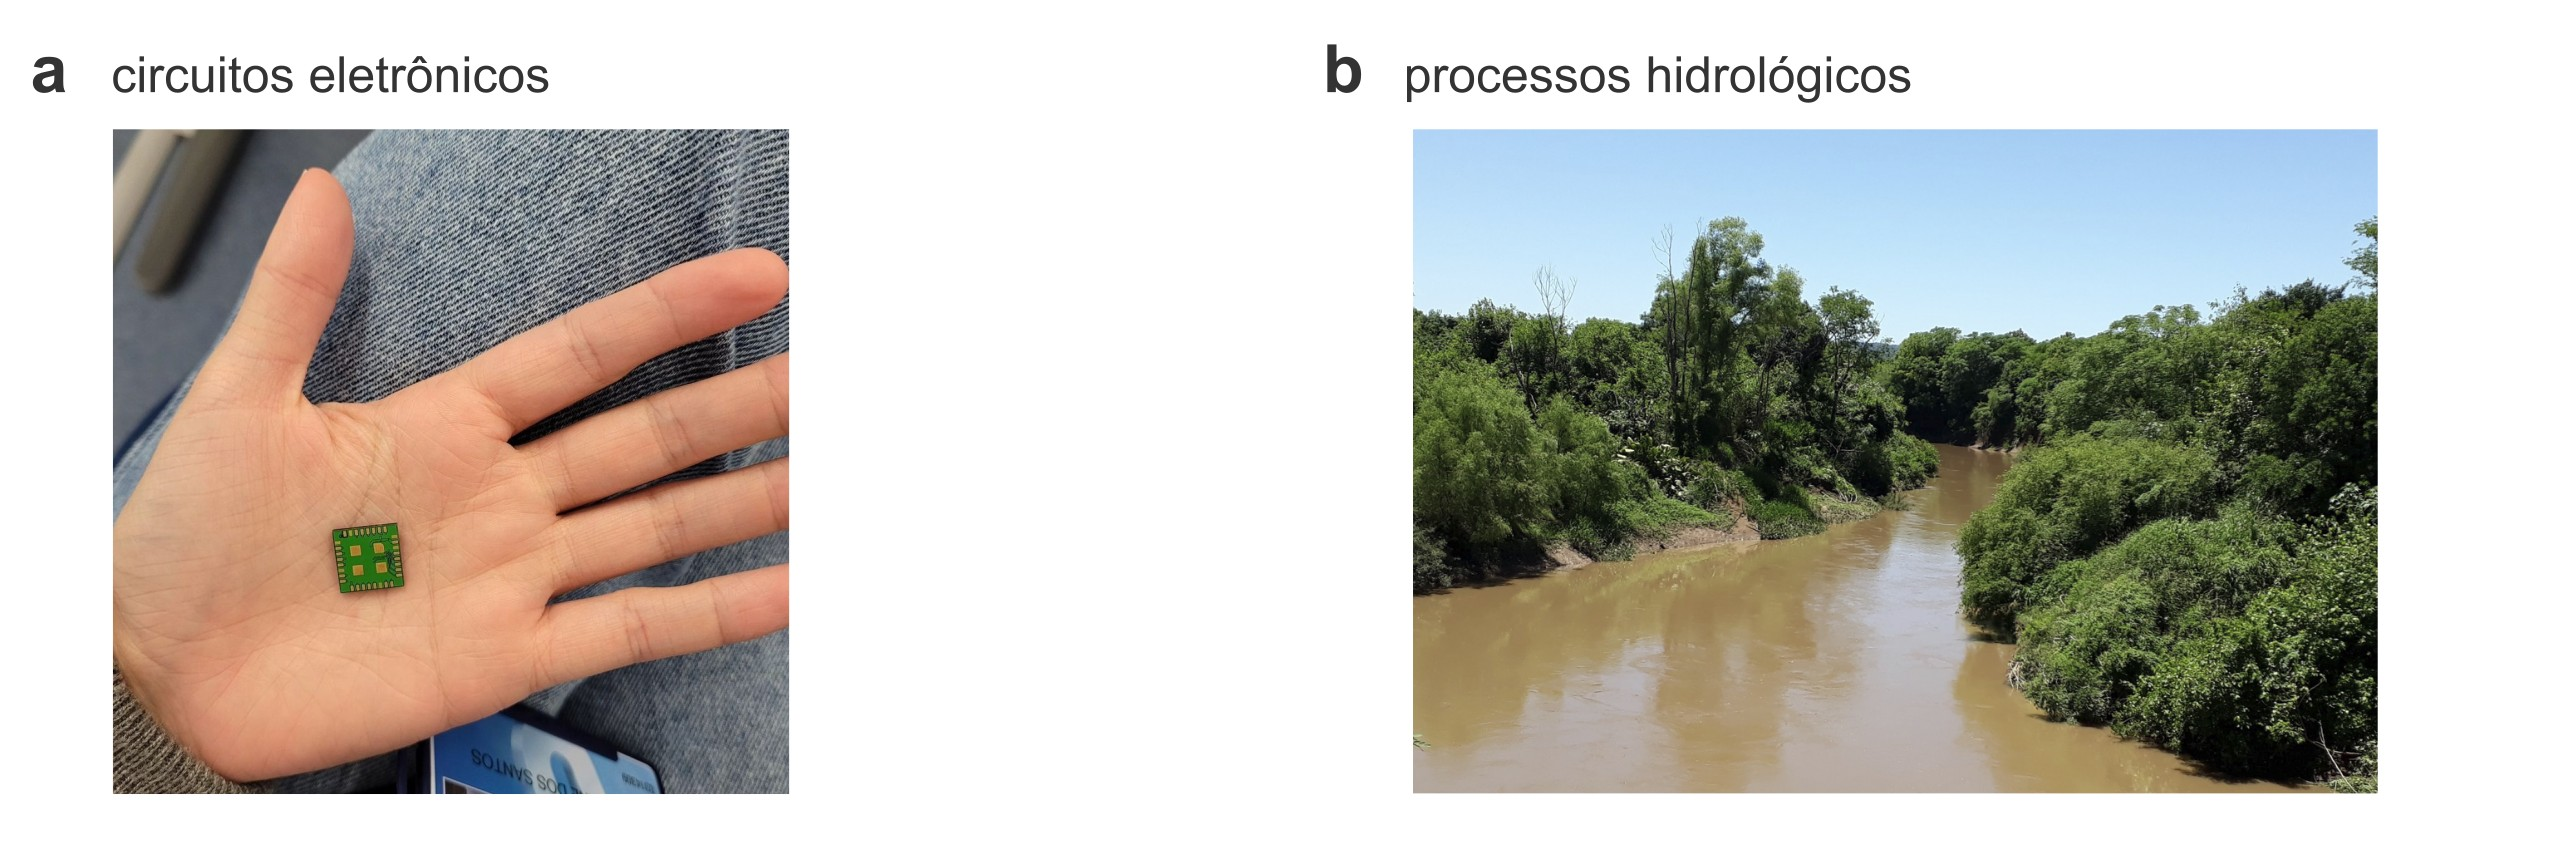
\includegraphics[width=0.95\linewidth]{fig_circuits.jpg}		
	\caption[De circuitos eletrônicos para processos hidrológicos]
	{\textbf{---\;De circuitos eletrônicos para processos hidrológicos.}
        \;\textbf{a.}\;---\;Aplicar um \gls{model} hidrológico consiste em \textit{literalmente} aplicar tensões em circuitos eletrônicos digitais. Os resultados das simulações se referem literal e objetivamente ao processamento dos estados binários de transistores. \;\textbf{b.}\;---\;Os usuários de modelos hidrológicos em geral aceitam que os resultados eletrônicos são uma \textit{representação realista}, ainda que aproximada, de diversos processos hidrológicos, seja a infiltração da chuva, o \gls{sf-runoff} ou a vazão de um rio. Como isso é possível? A fotografia em (\textbf{a}) foi cedida gentilmente pela engenheira eletricista Karina Kerne; a fotografia em (\textbf{b}) foi produzida pelo autor sobre a ponte sobre o Rio Pardinho ao sul do Lago Dourado, Santa Cruz do Sul, Rio Grande do Sul, Brasil.
	}
\label{fig:circuits}  % use qualitative label			
\end{figure}

\par Beven denomina essa filosofia implícita comum entre os usuários de modelos hidrológicos de \textbf{\gls{prag-realism}}. Ele classifica essa postura como ingênua, demonstrando que a tão almejada representação realista, quando levada a sério, torna-se um objetivo extraordinário diante da \textbf{\gls{uncert-empirical}} que existe na modelagem hidrológica. Se a gestão dos recursos hídricos deseja honestamente construir \textbf{\gls{ebp}}, o aconselhamento científico deve adotar uma \textit{postura crítica} em relação ao uso de modelos e de seus resultados. Como destacado por Ongaro e Andreoletti, a incerteza é um atributo pervasivo no processo de tomada de decisão \cite{Ongaro2022}. Nesse contexto, eles argumentam que o papel adequado das autoridades científicas é informar sobre as incertezas empíricas para que outros grupos de interesse\footnote{Tradução livre de \textit{stakeholders}, em inglês} possam deliberar sobre as incertezas éticas e as incertezas políticas em jogo. Mas essa postura crítica só é possível a partir de uma perspectiva filosófica explícita, denominada aqui de \textbf{\gls{instrument}}, que traz à tona diversos problemas que precisam ser endereçados antes de afirmarmos a correspondência entre campos eletromagnéticos em circuitos eletrônicos e processos hidrológicos em bacias hidrográficas. 

\par Com esse espírito, o objetivo deste capítulo é estabelecer os fundamentos filosóficos instrumentalistas que serão utilizados explicitamente ao longo desta tese. Irei aqui articular as seguintes questões da Filosofia da Ciência: o \gls{problem-just}, a epistemologia bayesiana, a \gls{falseabilidade} de teorias, o conceito de paradigmas e o \gls{problem-subdet}. A ontologia de modelos, que também é um tema pertinente, será tratada no próximo capítulo. Para os propósitos deste capítulo, deve-se considerar que \textbf{um \gls{model} é um veículo simbólico de uma teoria}. A intenção não é esgotar os temas apresentados (até porque isto iria demandar a escrita de muitas outras teses!). Ao contrário, deve-se entender o capítulo como uma visão panorâmica, como se estivéssemos no topo de uma montanha. Essa \gls{analogy} é particularmente útil, pois o cume propicia uma boa compreensão da paisagem que se estende abaixo de nossos pés. Ao mesmo tempo, é um território inóspito. O ar é rarefeito, sentimos vertigens. A locomoção é complicada, possível apenas por labirintos de trilhas cercadas de precipícios e cavernas. É preciso tomar cuidado para não se perder e nunca mais voltar.

\section{Justificação} \label{sec:epis:justific}

\par A \textbf{Epistemologia} é o ramo da Filosofia que investiga a natureza do próprio conhecimento humano. A pergunta epistemológica é: \textit{como é possível saber algo}? Por essa perspectiva, uma \textbf{\gls{teoria}} é um \textit{enunciado universal} que providencia uma explicação definitiva sobre determinado fenômeno. Dessa maneira, criar uma \gls{teoria} é relativamente fácil. Alguém pode professar, por exemplo, a \gls{teoria} que fadas da floresta são as responsáveis por fazer objetos domésticos desaparecerem, especialmente meias. Temos um fenômeno (o sumiço de coisas) e uma explicação definitiva (as fadas). A parte difícil, contudo, é \textit{justificar a verdade} de uma \gls{teoria} -- o assim denominado \textbf{\gls{problem-just}}. Aqui, a pergunta epistemológica fica um pouco mais complicada: \textit{como é possível saber algo \textbf{verdadeiro}}? No exemplo dado, se alguém alegar que, de fato, o cachorro é o responsável por fazer as meias sumirem, como defender a \gls{teoria} das fadas? Como separar o verdadeiro do falso? O exemplo das fadas da floresta pode, à primeira vista, parecer ridículo. Mas até poucos séculos pessoas eram torturadas e queimadas vivas em praça pública por questões como essa (especialmente as mulheres tidas como bruxas). Mesmo hoje, na verdade, é um assunto muito sério, com grandes implicações sociais e políticas. De acordo com Daniel Kahneman, as pesquisas no campo da psicologia demonstram que seres humanos exibem inúmeros \textbf{vieses cognitivos} que comprometem a sua capacidade de distinguir o verdadeiro do falso \cite{kahneman2011}.  

\par O problema epistemológico da justificação de teorias foi assimilado por duas correntes filosóficas diferentes durante o nascimento do \textbf{método científico} na modernidade \cite{sep-rationalism-empiricism}. Uma das correntes de pensamento, o \textbf{\gls{rationalism}}, sustenta que a \textit{Lógica} deve ser a justificativa para a verdade de teorias. Afinal, é claro que uma explicação incoerente não pode ser verdadeira. Essa posição costuma ser associada a Descartes (1596-1650), Spinoza (1632-1677) e Leibniz (1646-1716) -- os ditos racionalistas continentais. René Descartes, um dos maiores racionalistas de seu tempo, propagou a noção de que os sentidos são enganadores e elegeu a razão como guia de suas opiniões, estabelecendo um programa que ele chama de \textit{método da dúvida}. Em seu \textit{Discurso do método}\footnote{Descartes aprofunda suas ideias em \textit{Meditações}.}, ele chegou ao ponto de desconfiar da existência de tudo, alegando que a realidade pode ser indiscernível de um mero sonho \cite{descartes2008discurso}. Com isso, ele concluiu que o simples ato de \textit{duvidar} da existência garante ao menos uma única certeza absoluta: a existência de si mesmo\footnote{A ideia de Descartes de que se \say{penso, logo existo} (\textit{cogito, ergo sum}) garante a existência de um \textit{Self} que faz perguntas. Descartes tenta com isso provar a existência também de Deus. Mas a prova de Deus por Descartes é questionável, o que facilmente pode nos conduzir para o \textbf{solipsismo}: a tese de que o \textit{Self} está sozinho pairando no vazio, imaginando uma realidade que fundamentalmente não existe. Afinal, como \textit{você}, que está lendo esse texto, tem certeza que \textit{eu}, o autor, existo? Como garantir que todas as suas memórias não foram criadas agora, neste instante?  E se a sua vida inteira não for apenas uma alucinação imaterial?}. A outra corrente filosófica, o \textbf{\gls{empiricism}}\footnote{Tradução livre do termo em inglês \textit{empiricism}.}, defende que uma \gls{teoria} justifica-se por \textit{evidências empíricas}, ou seja, a partir de uma coleção de observações diretas de eventos e fenômenos. Essa linha de pensamento associa-se aos filósofos Locke (1632-1704), Hume (1711-1776) e Reid (1710-1796), os chamados empiristas britânicos. Locke, por exemplo, ficou conhecido por difundir as ideias de que todos nascem iguais como uma folha em branco, uma \textit{tabula rasa}, e adquirem conhecimento pela experiência, ao interagir com seu seu ambiente \cite{sep-locke}. 

\par Ainda que não sejam exatamente opostas, o que essas correntes filosóficas favorecem, em essência, são diferentes métodos de \textit{inferência}. Enquanto os racionalistas preferem a \textbf{\gls{infer-dedu}}, os empiristas preferem a \textbf{\gls{infer-indu}}. No primeiro caso, enunciados são justificados quando decorrem logicamente a partir de suas premissas, isto é, são deduzidos \cite{laird2010}. Por exemplo, considerando as premissas de que \say{\textit{todos os gaúchos gostam de mate}} e que \say{\textit{Clara é gaúcha}}, então deduzimos que \say{\textit{Clara gosta de mate}}. Geralmente o processo de \gls{infer-dedu} assume uma estrutura em que um enunciado condicional (se $S_1$ é verdade, então $S_2$ também é verdade) é seguido por uma sentença \textit{antecedente}, que pode ser uma afirmação (\textit{modus ponens}: $S_1$) ou uma negação (\textit{modus tollens}: $\neg S_1$), o que leva à conclusão da sentença \textit{consequente}. Na forma afirmativa (\textit{modus ponens}):
\begin{linenomath*}
    \begin{align*}
        S_1 \implies S_2 & \quad \textnormal{se alguém é gaúcho, então esse alguém gosta de mate} \\
        S_1 & \quad \textnormal{Clara é gaúcha}\\
        \therefore\;S_2 & \quad \textnormal{portanto, Clara gosta de mate}
    \end{align*}
\end{linenomath*}
A \gls{infer-dedu} garante a verdade da sentença consequente desde que suas premissas antecedentes sejam verdadeiras. No modo afirmativo ilustrado, ela vai no sentido de deduzir \textit{enunciados singulares} a partir de \textit{enunciados universais}. A \gls{infer-indu}, ao contrário, vai no outro sentido. Os empiristas buscam construir teorias (enunciado universais) \textit{generalizando} a partir de evidências (enunciados singulares) obtidas pela experiência empírica. Surge, assim, a noção de \textbf{\gls{hipotese}}: um esboço de \gls{teoria} a ser \textit{confirmado} ou \textit{verificado} pelas evidências. Por exemplo, se constatamos que os gaúchos que conhecemos gostam de beber mate, podemos inferir, por indução, que \textit{todos} gaúchos devem gostar de mate. Com um pouco mais de cautela e rigor empírico, eventualmente podemos afirmar que a \textit{probabilidade} de um gaúcho qualquer gostar de mate é alta, uma vez que em 99\% dos entrevistados em uma pesquisa com mil gaúchos afirmaram que sim, gostam de beber mate. A observação de fenômenos, para os empiristas, justifica a construção de generalizações que são plausíveis ou \textit{prováveis}.

\par Ambas as linhas de raciocínio são problemáticas. O uso estrito da Lógica como justificativa de teorias produz o \textbf{\gls{problem-regress}} \cite{cling2008}: se um enunciado $S_1$ é justificado por outro enunciado $S_2$ ($S_2 \implies S_1$), o que justifica $S_2$? Talvez o enunciado $S_3$ justifique $S_2$ e o enunciado $S_4$ justifique $S_3$, assim por diante, \textit{ad infinitum} ($\infty \implies ... \implies S3 \implies S_2 \implies S_1$). Uma alternativa é estabelecer um encadeamento circular de enunciados  ($S_1 \implies S_2 \implies S_3 \implies S_1$), mas isso é, em termos lógicos, ainda pior que a situação anterior, pois no final das contas os enunciados se auto-justificam. A regressão infinita é facilmente percebida quando crianças, sendo naturalmente curiosas, aprendem a perguntar \say{\textit{porquê?}}. É possível parar a regressão (ou pelo menos \textit{parar as perguntas}) ao se estabelecer verdades fundamentais, axiomas inquestionáveis, como acontece na Matemática. Mas na Ciência isso apenas produz teorias \textit{dogmáticas}, baseadas em convenções relativamente arbitrárias, que são alvos fáceis para as críticas dos empiristas. Por outro lado, o uso da experiência empírica como justificativa de teorias traz consigo um problema insolúvel, descrito por David Hume (1711-1776) e conhecido hoje como \textbf{\gls{problem-indu}}. A \gls{infer-indu} é frágil porque ela se fundamenta no \textbf{\gls{principio-uniform}}: a suposição de que as regularidades da natureza observadas no passado serão as mesmas a serem observadas no futuro. Essa suposição é a base de toda a Física, afinal, as leis observadas hoje são frequentemente usadas para prever eventos no futuro e reconstruir os eventos que já ocorreram. Apesar de intuitivo, não é possível justificar racionalmente o \gls{principio-uniform}. Se evocarmos o fato de que desde sempre ele demonstrou-se funcional ou correto, incorremos em um argumento circular, logicamente inválido, que \textit{evoca o próprio \gls{principio-uniform} para justificar o princípio da uniformidade} \cite{sep-induction-problem}. Em outras palavras, não se pode defender a \gls{infer-indu} através de um argumento indutivo! Assim, o \gls{principio-uniform} é, em última instância, o dogma fundamental dos empiristas \footnote{As ideias de Hume nos conduzem inevitavelmente para o \textbf{ceticismo}. Além do \gls{problem-indu}, Hume argumentou que a \textbf{causalidade} entre fenômenos é um conceito imaginário, jamais experienciado \textit{diretamente} na realidade. Imagine que uma bola de bilhar colida com outra bola em repouso. A seguir, a bola em repouso passa se mover também. Newton diria que isso aconteceu \textit{por causa} da lei conservação de movimento. Mas essa lei requer diversos conceitos teóricos imaginados, como massa e energia. O que de fato podemos experienciar são eventos ocorrendo um após o outro, mas nunca a conexão de causa e efeito entre eles. Para Hume, \textit{essa conexão não existe}. }.    

\par O avanço da modernidade gradualmente reduziu a rivalidade intelectual existente entre os pensadores do continente europeu e as ilhas britânicas. O \gls{empiricism}, ainda que revisado e moderado, triunfou sobre o \gls{rationalism} -- especialmente após a obra de Immanuel Kant (1724-1804). Em sua \textit{Crítica à Razão Pura} (1781), esse pensador propõe uma síntese entre \gls{rationalism} e \gls{empiricism} \sethlcolor{pink}\hl{[todo:cite]}. Nela, Kant concorda com os empiristas -- de que a experiência empírica justifica o conhecimento -- mas faz uma concessão ao \gls{rationalism}, estabelecendo que conceitos teóricos sobre os objetos a serem conhecidos são necessários \textit{a priori}. Sem o que ele denominava de \textit{categorias transcendentais}, não temos muito o que fazer com as percepções que coletamos sobre o mundo externo. A hegemonia do \gls{empiricism} na modernidade  acabou culminando no início do século XX com o movimento filosófico do \textbf{\gls{positivismo}}. Esse movimento estabeleceu o senso comum de que teorias científicas são \textit{verificadas} ou \textit{confirmadas} a partir da coleta de observações e análises estatísticas. Mas essa concepção foi ultrapassada a partir de meados do século XX, principalmente em razão das transformações impressionantes na Física. Isso reanimou o debate sobre como que a Ciência justifica suas teorias e muda elas no longo prazo, com novas perspectivas sendo propostas por Karl Popper (1902-1994) e Thomas Kuhn (1922-1996), criando as condições para o debate contemporâneo na Filosofia da Ciência: o \gls{realism-sci} e o propósito da Ciência.

\section{Confirmação} \label{sec:epis:bayes}

\par Na seção anterior, vimos que a corrente empirista estabelece que uma \gls{hipotese} representa um esboço de \gls{teoria} que deve ser \textit{confirmada} pelas experiência empírica. Nesse sentido, as ideias do filósofo e estatístico Thomas Bayes (1701-1761) fornecem um método de \gls{infer-indu} particularmente útil para a confirmação de hipóteses a partir da matemática das probabilidades \cite{sep-epistemology-bayesian}, \cite{sprenger2019}. A ideia central da chamada \textbf{epistemologia bayesiana} professa que o conhecimento não é uma questão de tudo ou nada, preto ou branco, mas que apresenta sutilezas, com diversos tons de cinza entre o verdadeiro e o falso. A razão disso deriva do reconhecimento de que as observações empíricas estão inevitavelmente sujeitas a um \textit{ruído aleatório}, ou seja, de que existe \textbf{\gls{uncert-stats}} nos dados amostrados. Para essa corrente empirista, as sutilezas do conhecimento consistem no \textbf{\gls{grau-convic}} \footnote{Tradução livre do termo \textit{credence} do inglês.} na verdade de uma \gls{hipotese}. Esse \gls{grau-convic} deve ser atualizado à medida que evidências favoráveis ou desfavoráveis são obtidas pela experiência empírica. 

\par Antes prosseguir, será útil estabelecer um exemplo intuitivo. 

\par Considere que você está em no aeroporto de um país distante, na praça de alimentação de um agitado terminal internacional. Você deseja saber se a pessoa na mesa à sua frente vai pegar o seu mesmo voo para o Brasil. Sem nenhuma informação disponível, o seu \gls{grau-convic} nessa \gls{hipotese} é relativamente baixo, pois existem dezenas de voos previstos neste terminal para diversos outros países. Mas se você desconfia que ela é brasileira, o seu \gls{grau-convic} aumenta – afinal, seu voo deve estar lotado de outros brasileiros. Ao mesmo tempo, é preciso ter cautela, pois ser brasileiro não implica necessariamente estar viajando para o Brasil. E mesmo que a pessoa não fosse brasileira, também existiria a pequena chance de estar viajando para o Brasil no mesmo voo que você, a turismo ou a negócios. Um fato é certo: \textit{uma evidência favorável de que ela é brasileira fará você atualizar o seu grau de convicção}. A epistemologia bayesiana articula como fazer isso de forma matematicamente precisa.

\par Um bom ponto de partida para formalizar o conceito de \gls{grau-convic} em termos de probabilidades é notar que uma dada \gls{hipotese} $H$ e a sua evidência favorável $E$ se distribuem em um \textbf{\gls{espaco-possib}} $\Omega$. Na perspectiva bayesiana, se atribui para cada uma dessas possibilidades um \gls{grau-convic} que pode ser considerado probabilístico desde que elas sejam \textit{mutuamente excludentes} (não podem ser verdadeiras ao mesmo tempo) e \textit{conjuntamente exaustivas} (pelo menos uma delas é verdadeira). Dadas essas condições, se observa então o \textbf{\gls{princip-prob}} a partir dos seguintes axiomas:
\begin{itemize}
    \item \textbf{Não-negatividade}. A probabilidade de uma dada possibilidade $A$ deve ser um número real não-negativo: $P(A) \geq 0$;
    \item \textbf{Normalização}. As probabilidades de todas as possibilidades devem somar até a unidade: $P(\Omega) = 1$, e;
    \item \textbf{Aditividade}. Por serem incompatíveis, a probabilidade de duas possibilidades $A$ e $B$ é a soma das suas probabilidades individuais: $P(A \cup B ) = P(A) + P(B)$.
\end{itemize}

\par No exemplo do aeroporto, essas possibilidades são quatro: a pessoa é brasileira e está no mesmo voo ($E$ é verdadeira e $H$ é verdadeira); a pessoa é brasileira e não está no mesmo voo ($E$ é verdadeira e $H$ é falsa); a pessoa não é brasileira e está no mesmo voo ($E$ é falsa e $H$ é verdadeira), e; a pessoa não é brasileira e não está no mesmo voo ($E$ é falsa e $H$ é falsa). Esse \gls{espaco-possib} pode ser visualizado mais facilmente a partir de uma tabela com números ilustrativos, como na Tabela\,\ref{tbl:bayes-aeroporto}. Assim sendo, considere que no terminal internacional existem previstos 200 voos (apenas um deles para o Brasil) e que cada avião comporta 500 passageiros. Ou seja, no total existem 100 mil passageiros circulando no terminal. Além disso, existem 800 brasileiros no terminal, sendo 450 no seu voo e outros 350 com outros destinos.
\begin{table}[ht]
     % placed on top of page    
    \centering	
    \small
    \sffamily
    \begin{tabular}{ l  c  c  c} % preset number of columns and aligment
       & \textbf{mesmo voo ($H$)} & \textbf{outro voo ($\neg H$)} & totais\\  
        \hline
        \textbf{é brasileira ($E$)} & 450 & 350 & 800\\
        \textbf{não é brasileira ($\neg E$)} & 50 & 99150 & 99200\\
        \hline
        totais & 500 & 99500 & 100000\\
    \end{tabular}
    \caption[Espaço de possibilidades do exemplo do aeroporto]{Espaço de possibilidades do exemplo do aeroporto. Os números representam a distribuição de passageiros nas diferentes combinações entre \gls{hipotese} $H$ (vai no mesmo voo) e evidência $E$ (nacionalidade é brasileira)}
    \label{tbl:bayes-aeroporto}
\end{table} 

A inspeção da tabela nos permite facilmente perceber que a probabilidade da sua \gls{hipotese} ser verdadeira, de um passageiro qualquer estar no seu voo, é de $P(H) = 0.005$ (0.5\%), pois $500 / 100000 = 0.005$. No jargão bayesiano, essa é a \textbf{\gls{prior}} \footnote{Tradução livre do inglês do termo \textit{prior}}. Mas a evidência de que essa pessoa pode ser brasileira muda tudo. Agora, a probabilidade da sua \gls{hipotese} ser verdadeira dado que a evidência é verdadeira é de $P(H | E) = 0.56$ (56\%), pois $450 / 800 = 0.56$. No jargão bayesiano, essa é a \textbf{\gls{posterior}} \footnote{Tradução livre do inglês do termo \textit{posterior}}. O \textbf{\gls{bayes-theorem}} formaliza esse raciocínio:
\begin{linenomath*}
\begin{equation}
\label{eq:bayes}
    P(H | E) = \frac{P(H) \cdot P(E | H)}{P(E)}
\end{equation}
\end{linenomath*}
Em que $P(H | E)$ é a probabilidade da \gls{hipotese} $H$ ser verdadeira dado que a evidência $E$ é verdadeira (probabilidade posterior); $P(H)$ é a probabilidade da \gls{hipotese} $H$ ser verdadeira (probabilidade anterior);  $P(E | H)$ é a probabilidade da evidência $E$ ser verdadeira dado que a \gls{hipotese} $H$ é verdadeira, chamada de \textbf{\gls{likelihood}}, e; $P(E)$ é a probabilidade da evidência ser verdadeira sob todas as possibilidades. No caso do aeroporto:
\begin{linenomath*}
\begin{equation*}
    P(H | E) = \frac{\frac{500}{100000} \cdot \frac{450}{500}}{\frac{800}{100000}} = \frac{450}{800} = 0.56\,(56\%)
\end{equation*}
\end{linenomath*}
O que o Teorema de Bayes quer dizer é que a estimativa da probabilidade da \gls{hipotese} ser verdadeira diante da evidência favorável deve levar em consideração tanto o \gls{espaco-possib} reduzido \textit{que a evidência favorável implica} (no exemplo, o fato de existirem poucos brasileiros no terminal internacional) quanto de que existe a chance \textit{da evidência não garantir a hipótese} (no exemplo, o fato de que nem todos no seu voo são brasileiros).  Ou simplesmente:
\begin{linenomath*}
\begin{equation*}
    \text{Posterior} = \text{Anterior} \times \text{Verossimilhança} \div \text{Evidência}
\end{equation*}
\end{linenomath*}

\par A atualização do \gls{grau-convic} só é possível \textit{desde que} a evidência favorável à \gls{hipotese} seja verdadeira. Por essa razão, esse é o chamado \textbf{\gls{princip-cond}} da epistemologia bayesiana. No exemplo do aeroporto, tudo é muito óbvio porque os números absolutos de passageiros foram fornecidos pela tabela. As probabilidades calculadas dessa forma são objetivas, baseadas na \textit{frequência} de cada conjunto do \gls{espaco-possib} $\Omega$. Mas em uma situação prática geralmente só temos acesso aos graus de convicção do \gls{espaco-possib} $\Omega$, que devem mudar à medida que novas evidências são obtidas. Para manter a concordância com os axiomas do probabilismo, a condicionalização ou \textbf{\gls{conditioning}} \footnote{O termo \textit{condicionamento} e \textit{condicionalização} serão utilizados aqui de forma equivalente.} com as evidências deve \textit{zerar}, \textit{escalonar} e \textit{normalizar} os valores das probabilidades. No exemplo do aeroporto, quando descobrimos que a pessoa no aeroporto é definitivamente brasileira, devemos zerar as probabilidades de que ela não é brasileira, o que implica escalonar proporcionalmente a probabilidade das outras possibilidades e \textit{normalizar seus valores} de forma que a sua soma seja igual à unidade, pois $P(\Omega) = 1$. Por outro lado, se apenas inferirmos que a pessoa na mesa à frente fala português (talvez por estar lendo algum livro), isso não é suficiente para zerar a probabilidade dela não ser brasileira (afinal, outras nacionalidades também falam português!).

\begin{table}[t]
     % placed  here
    \centering	
    \small
    \sffamily
    \rowcolors{2}{white}{rowgray}
    \begin{tabular}{ l c c c c c } % preset number of columns and aligment
        \toprule
        \textbf{Hipótese \textit{i}} & \textbf{$P(H_i)$} & \textbf{$P(E | H_i)$} & \textbf{$P(H_i) \cdot P(E | H_i)$} & \textbf{$P(H_i | E)$}\\ 
        \midrule
        $H_1$: $X < x_1$ & 0.143 & 0.008 & 0.001 & 0.008\\ 
        $H_2$: $x_1 \leq X < x_2$ & 0.143 & 0.026 & 0.004 & 0.026\\ 
        $H_3$: $x_2 \leq X < x_3$ & 0.143 & 0.084 & 0.012 & 0.084\\ 
        $H_4$: $x_3 \leq X < x_4$ & 0.143 & 0.171 & 0.024 & 0.171\\ 
        $H_5$: $x_4 \leq X < x_5$ & 0.143 & 0.208 & 0.03 & 0.208\\ 
        $H_6$: $x_5 \leq X < x_6$ & 0.143 & 0.275 & 0.039 & 0.275\\ 
        $H_7$: $X \geq x_6$ & 0.143 & 0.227 & 0.032 & 0.227\\ 
        \midrule
        totais & 1.0 & 1.0 & 0.14 & 1.0\\
        \bottomrule
    \end{tabular}
    \caption[Exemplo \gls{conditioning} objetivo]{
    Exemplo ilustrativo do \gls{conditioning} da distribuição de probabilidade de uma variável aleatória $X$. Nesse a distribuição anterior $P(H)$ foi definida como uniforme pela observação do \gls{princip-indif} (bayesianismo objetivo).
    }
    \label{tbl:objective}
\end{table} 

\begin{table}[t]
     % placed  here
    \centering	
    \small
    \sffamily
    \rowcolors{2}{white}{rowgray}
    \begin{tabular}{ l  c  c  c  c c} % preset number of columns and aligment
        \toprule
        \textbf{Hipótese \textit{i}} & \textbf{$P(H_i)$} & \textbf{$P(E | H_i)$} & \textbf{$P(H_i) \cdot P(E | H_i)$} & \textbf{$P(H_i | E)$}\\ 
        \midrule
        $H_1$: $X < x_1$ & 0.227 & 0.008 & 0.002 & 0.022\\ 
        $H_2$: $x_1 \leq X < x_2$ & 0.273 & 0.026 & 0.007 & 0.088\\ 
        $H_3$: $x_2 \leq X < x_3$ & 0.229 & 0.084 & 0.019 & 0.236\\ 
        $H_4$: $x_3 \leq X < x_4$ & 0.146 & 0.171 & 0.025 & 0.306\\ 
        $H_5$: $x_4 \leq X < x_5$ & 0.082 & 0.208 & 0.017 & 0.208\\ 
        $H_6$: $x_5 \leq X < x_6$ & 0.036 & 0.275 & 0.01 & 0.12\\ 
        $H_7$: $X \geq x_6$ & 0.008 & 0.227 & 0.002 & 0.022\\ 
        \midrule
        totais & 1.0 & 1.0 & 0.08 & 1.0\\
        \bottomrule
    \end{tabular}
    \caption[Exemplo de \gls{conditioning} subjetivo]{
    Outro exemplo ilustrativo do \gls{conditioning} da distribuição de probabilidade de uma variável aleatória $X$. Nesse caso a distribuição anterior $P(H)$ foi definida subjetivamente, por opinião especialista (bayesianismo subjetivo).
    }
    \label{tbl:subjective}
\end{table}

\par O \gls{princip-cond} concede que se aplique o Teorema de Bayes para um número finito de $N$ hipóteses $H_1$, …, $H_N$, desde que elas sejam possibilidades mutuamente excludentes e conjuntamente exaustivas. Nesse caso, o Teorema de Bayes assume a seguinte forma:
\begin{linenomath*}
\begin{equation}
\label{eq:bayes-finite}
    P(H_i | E) = \frac{P(H_i) \cdot P(E | H_i)}{\sum_{j=1}^{N}P(E | H_j) \cdot P(H_j)}
\end{equation}
\end{linenomath*}
O denominador nessa equação é uma constante que desempenha o papel de normalizar os valores das probabilidades,  assegurando que $P(\Omega) = 1$. Aqui, nota-se que a normalização oportuniza se atribuir graus de convicção \textit{não probabilísticos} para a \gls{likelihood} $P(E | H)$ sem violar o \gls{princip-prob}, desde que sejam valores não-negativos. Ou seja, a \gls{likelihood} $P(E | H)$ pode ser interpretada como um \textit{peso} fornecido pelas evidências. Se for o caso, a notação da \gls{likelihood} deve ser modificada para uma \textbf{função de \gls{likelihood} informal}, denotada por $\mathcal{L}(E|H)$\footnote{Essa é a base do método \acrfull{glue} para análises de incertezas, introduzido no próximo capítulo}. De uma forma ou de outra, a distribuição de \gls{posterior} de uma variável aleatória deve ser condicionalizada por uma distribuição de probabilidade (ou de pesos) estimada empiricamente. Para tanto, é preciso discretizar os valores da variável em $N$ intervalos, que são as hipóteses $H_1$, …,$H_N$ da Equação \eqref{eq:bayes-finite}. Para cada \gls{hipotese} $H_i$, deve-se atribuir inicialmente a sua \gls{prior} $P(H_i)$. A seguir, evidências empíricas devem ser obtidas para se obter a \gls{likelihood} $P(E | H_i)$ de cada \gls{hipotese}. A \gls{posterior} de cada \gls{hipotese} então é condicionalizada através da aplicação da Equação \eqref{eq:bayes-finite}. Por fim, se considerarmos a distribuição posterior obtida como a distribuição anterior da próxima etapa, a confirmação da distribuição de probabilidade da variável ocorre incrementalmente à medida que novas evidências se acumulam. A Tabela \ref{tbl:objective} mostra um exemplo do \gls{conditioning} da distribuição de probabilidade de uma variável aleatória $X$, que no caso foi dividida em sete intervalos discretos delimitados pelos limiares $x_1, ..., x_6$.

\par Uma questão controversa no processo de \gls{conditioning} é a definição das probabilidades anteriores na primeira etapa de todas, quando ainda não existem evidências. No caso da Tabela \ref{tbl:objective}, qual é a justificativa para a distribuição de \gls{prior} $P(H_i)$ ser uniforme? Esse é o dito \textbf{\gls{problem-priors}} na epistemologia bayesiana, que divide o campo em duas principais correntes de bayesianismo: a \textit{subjetiva} e a \textit{objetiva}. Para avançar, é preciso decidir entre uma das duas. Por um lado, a corrente do \textbf{\gls{bayes-sub}} admite qualquer distribuição de \gls{prior} desde que ela não viole o \gls{princip-prob}. O problema óbvio aqui é tornar a distribuição posterior mais sensível aos valores da distribuição anterior do que aos da própria evidência, como demonstrado na Tabela \ref{tbl:subjective}. A Figura \ref{fig:bayes} deixa clara diferença entre os resultados posteriores $P(H | E)$ entre as Tabelas \ref{tbl:objective} e \ref{tbl:subjective}, ainda que tenham sido usadas exatamente a mesma distribuição de \gls{likelihood} $P(E | H)$ para o \gls{conditioning}. A defesa dessa corrente sustenta que é legítimo que diferentes opiniões subjetivas possam ser comparadas objetivamente. Além disso, se as evidências forem consistentes, opiniões divergentes sobre a distribuição anterior tornam-se irrelevantes no longo prazo, se dissipando durante as sucessivas etapas de \gls{conditioning}. Por outro lado, a corrente do \textbf{\gls{bayes-obj}} prefere eliminar todo e qualquer viés ao se definir a distribuição anterior. Nesse intuito, se recomenda o \textbf{\gls{princip-indif}}: o \gls{grau-convic} em duas ou mais hipóteses deve ser igual na ausência de razões suficientes para o contrário. No caso na Tabela \ref{tbl:objective},  talvez não existam motivos suficientes para diferenciar os valores de $P(H_i)$ e por isso foi adotada uma distribuição uniforme. Esse princípio pode até parecer natural, mas ele não passa de uma convenção arbitrária: diante da completa ignorância, qualquer distribuição de \gls{prior} é igualmente provável, sendo a distribuição uniforme na verdade um caso extremamente específico.

% figure
\begin{figure}[t!] % place figure in the page
	\centering				
	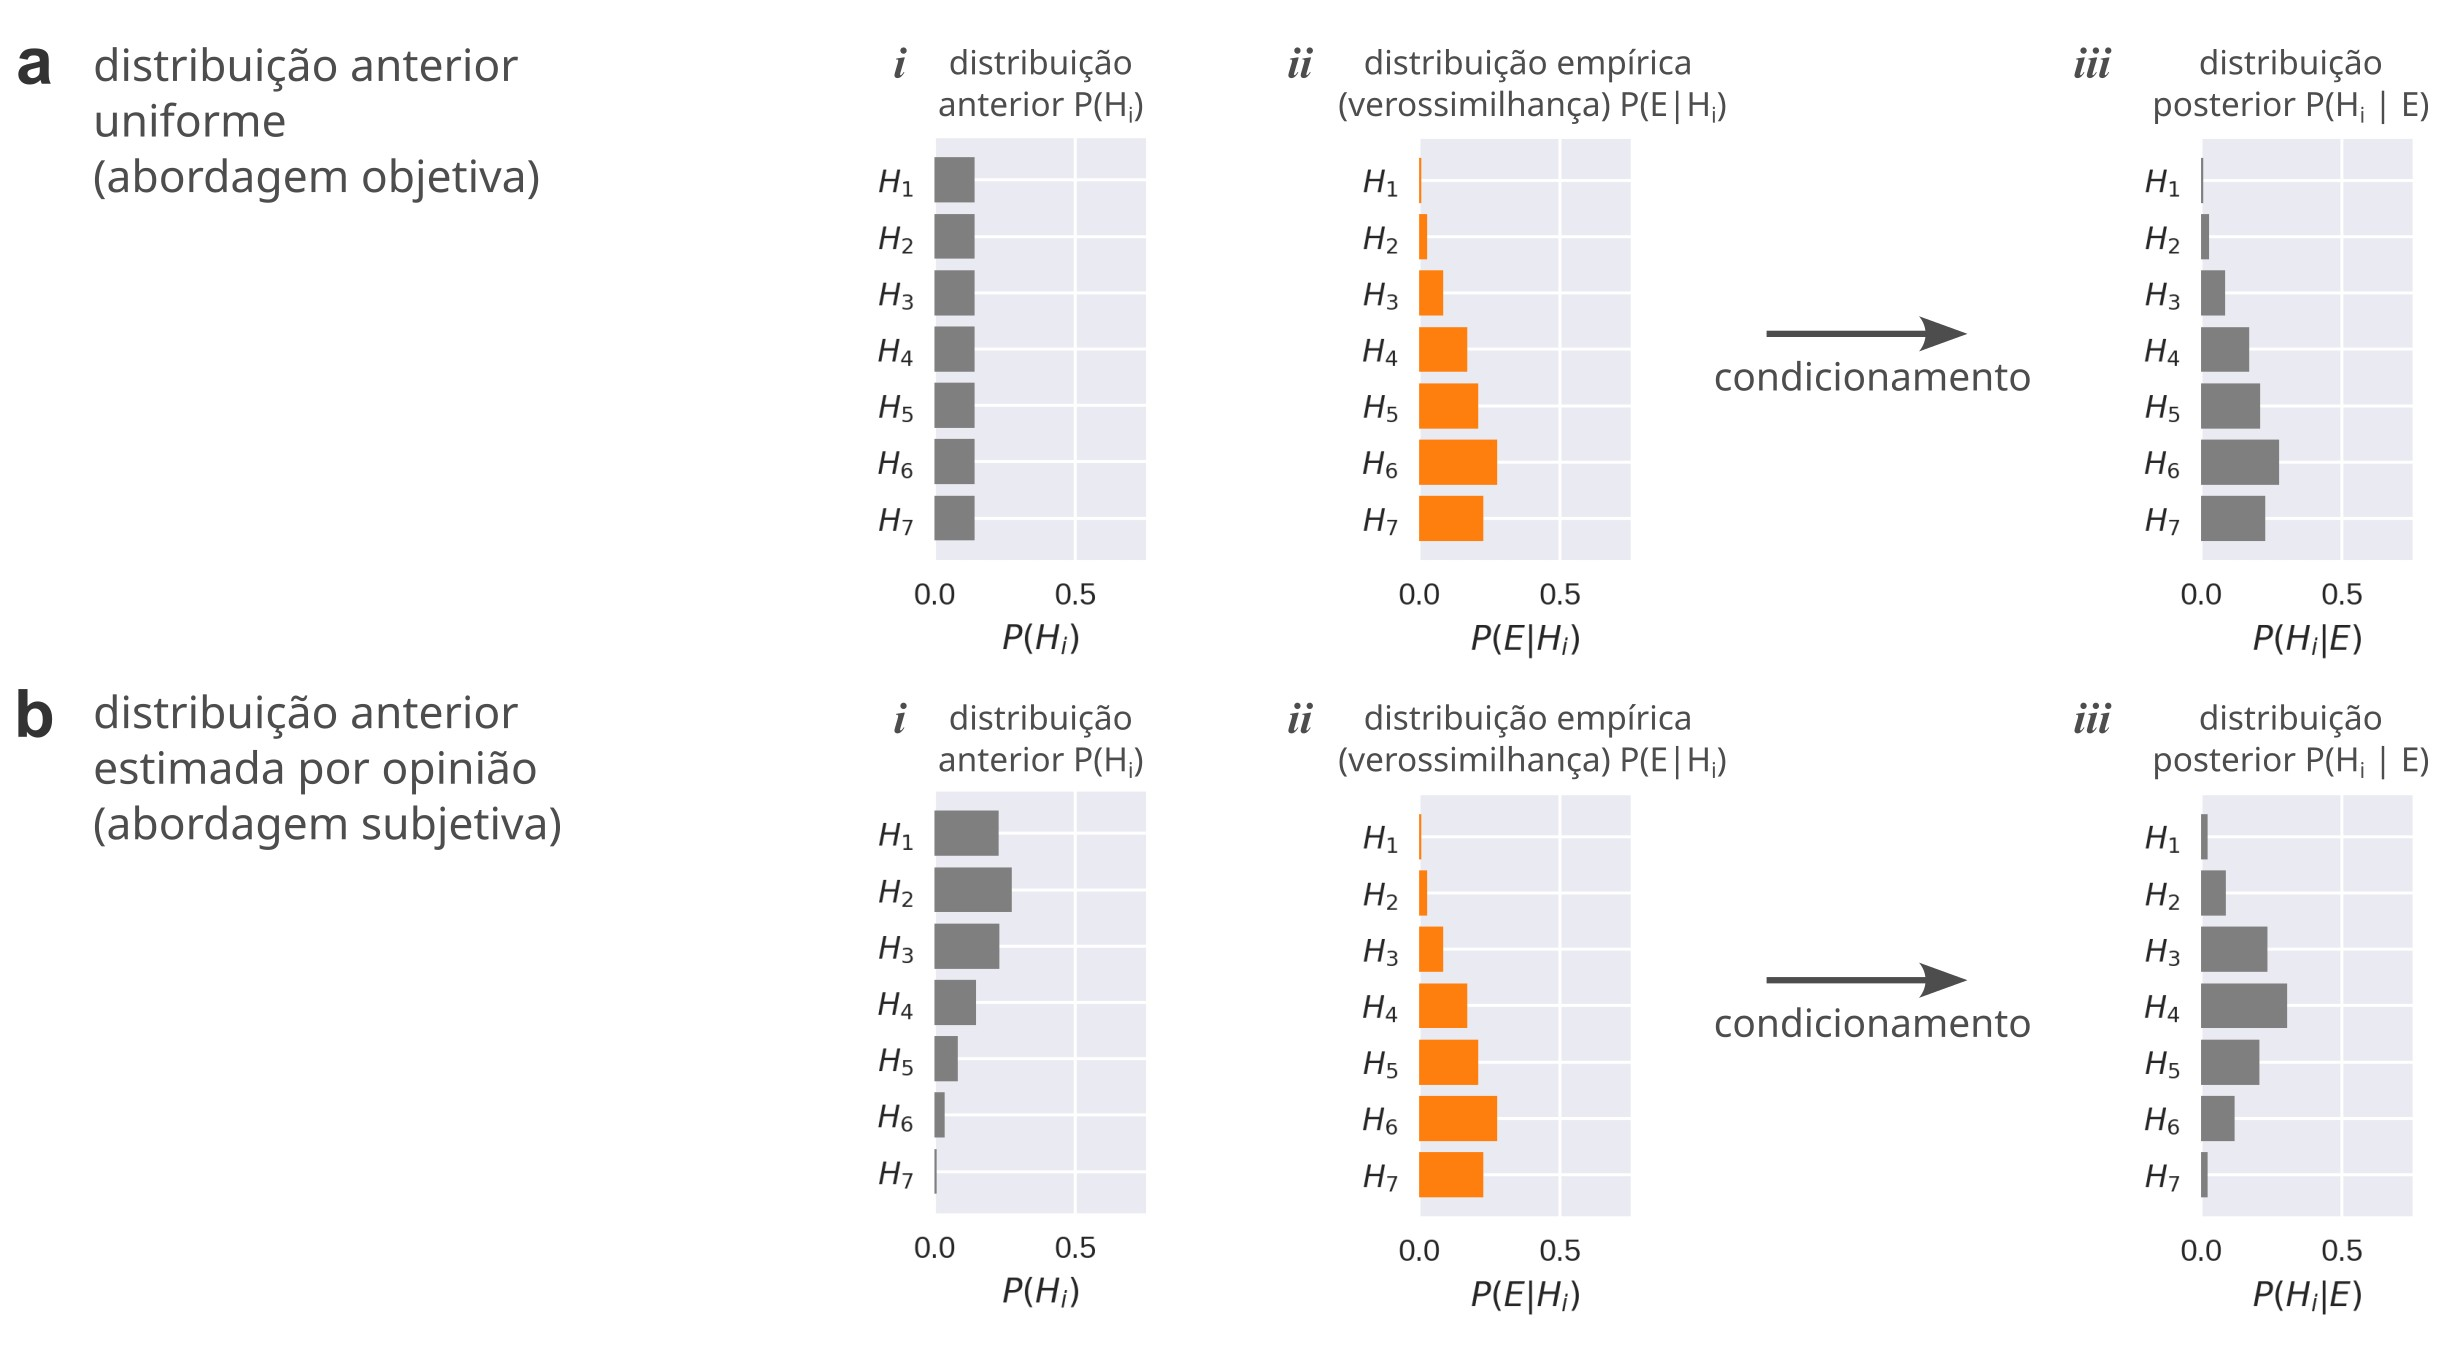
\includegraphics[width=0.95\linewidth]{fig_bayes.jpg}		
	\caption[Exemplo do \gls{conditioning} bayesiana]
	{\textbf{---\;Condicionamento da distribuição anterior de uma variável aleatória.}
        Aqui são apresentados visualmente os dados ilustrativos das Tabelas \ref{tbl:objective} e \ref{tbl:subjective}. Em ambos os casos a evidência é a mesma, o que muda são as premissas utilizadas na distribuição anterior. \;\textbf{a}\;---\;Distribuição uniforme, considerando o \textit{princípio da indiferença} do \gls{bayes-obj}. \;\textbf{b}\;---\;Distribuição definida por opinião, prática considerada válida no \gls{bayes-sub}.  
	}
\label{fig:bayes}  % use qualitative label			
\end{figure}

\par Outra questão em aberto no processo de \gls{conditioning} é como se obter a \gls{likelihood} $P(E | H)$ a partir das evidências. Afinal, sem detalhes precisos sobre todo o \gls{espaco-possib} $\Omega$, como no exemplo do aeroporto, as evidências em geral consistem em dados amostrados que não se traduzem automaticamente em probabilidades. Isso se agrava ainda mais no caso de uma variável aleatória contínua, quando buscamos estimar uma distribuição de probabilidades a partir dos dados disponíveis. Assim como no \gls{problem-priors}, a solução para essa questão requer uma tomada de decisão, que é se estabelecer um conjunto de premissas sobre \textit{o comportamento do ruído aleatório}\footnote{Um fato irônico da abordagem bayesiana é que a \gls{hipotese} sobre o comportamento do ruído só pode ser justificada pela lógica, nunca pelas evidências, sob pena de se adentrar em uma regressão infinita de decisões sobre o ruído do ruído. Afinal, para justificar com base em evidências a \gls{hipotese} sobre o ruído aleatório, teríamos que repetir o método bayesiano \textit{ad infinitum}, avaliando o ruído do ruído, e o ruído do ruído do ruído, assim por diante.}. Nesse rumo, um exemplo particularmente útil para nossa discussão futura sobre modelos hidrológicos é o ajuste de curvas matemáticas que relacionam dois fenômenos, como no caso da \textbf{\gls{rating-curve}} que descreve a vazão em função do nível observado em uma seção de rio (ver Destaque \ref{box:rating-curve}).  Nesse caso, a curva matemática consiste na \gls{hipotese}, ou \textbf{\gls{model}}, que estamos interessados em saber o \gls{grau-convic}.  Uma relação geral para esse problema é a seguinte \cite{Box1979}:
\begin{linenomath*}
\begin{equation}
\label{eq:bayes-model}
    O(x, t) = M(x, t, \Theta) + \varepsilon(x, t)
\end{equation}
\end{linenomath*}
Em que $O(x, t)$ é a observação empírica obtida na variável independente $x$ e no tempo $t$; $M(x, t, \Theta)$ são as predições do \gls{model} $M$ em $x,t$ dado o vetor de \gls{parameters} $\Theta$, e; $\varepsilon(x, t)$ é o \textbf{erro}\footnote{Também denominado de \textbf{resíduo}.} da observação empírica em $x,t$. É claro que, nesse contexto, as variáveis aleatórias de interesse para se estimar a \gls{likelihood} do \gls{model} $M$ são os próprios \gls{parameters} $\Theta$. Um conjunto de premissas típicas\footnote{A introdução de viés, autocorrelação no tempo e outras distribuições também podem ser feitas dentro de um tratamento matematicamente formal, ainda que mais intricado.} sobre o comportamento do ruído aleatório é que o erro $\varepsilon$ apresenta:
\begin{enumerate}
    \item média zero, isto é, $\mu_{\varepsilon} = 0$;
    \item variância $\sigma_{\varepsilon}^2$ constante (estável);
    \item independência no tempo, e;
    \item distribuição normal: $p(\varepsilon) = \frac{1}{\sigma_{\varepsilon} \sqrt{2\pi}}e^{-(\varepsilon-\mu_{\varepsilon})^2/{(2\sigma_{\varepsilon}^2)}}$, em que $\mu_{\varepsilon}$ é a média do erro (zero) e $\sigma_{\varepsilon}$ é o desvio padrão do erro.
\end{enumerate}
A justificativa racional para considerar a distribuição normal se fundamenta no \textbf{\gls{theorem-central-limit}}, que estabelece que a média amostral de uma população qualquer é uma população normalmente distribuída\footnote{O que esse teorema quer dizer é que somas de números aleatórios (note que a média é uma soma) tendem a produzir naturalmente o padrão da curva normal pela simples combinação de valores altos com valores baixos. Por exemplo, considere o lançamento de um dado não enviesado de seis faces. A probabilidade de cada face superior apresentar um dos valores do conjunto $\{1, 2, 3, 4, 5, 6\}$ é a mesma, de $1/6$. Mas a probabilidade da \textit{média} dos valores amostrados em $n$ lançamentos tende a ser muito maior entre valores intermediários à medida que $n$ cresce, pois valores altos são compensados por valores baixos. É esse o fato que produz o padrão de sino invertido modelado pela curva normal.}. Com isso, o problema da \gls{likelihood} dos \gls{parameters} $\Theta$ se resolve ao se estimar a variância populacional do erro $\sigma^2_\varepsilon$ pela sua variância amostral, que é definida por $s^2_{\varepsilon} = \frac{1}{df}\sum_{i=1}^{n}({\varepsilon_i - \bar{\varepsilon}})^2$, em que $\bar{\varepsilon}$ é a média amostral do erro; $n$ é o tamanho amostral, e; $df$ é o número de graus de liberdade\footnote{$df = n-2$ para modelos com dois \gls{parameters}.} \cite{graybill1994}. O erro $\varepsilon_i$ de cada $n$ observação é a diferença entre a observação $O_i$ e a predição da curva do \gls{model} $M_i$ definida por \gls{parameters} $\Theta$ ajustados com técnicas de otimização, como o método dos mínimos quadrados. A seguir, a incerteza associada à variância do erro deve ser assimilada de alguma forma pelos \gls{parameters} $\Theta$. Para modelos lineares, é possível fazer isso analiticamente, a partir dos princípios da combinação linear de variáveis aleatórias. Uma alternativa robusta, aplicável para modelos em geral, é o método das \textbf{\gls{monte-carlo}}. Nesse método, são feitas inúmeras \textit{reamostragens} do erro $\varepsilon$, ou seja, simulações de realizações estatisticamente equivalentes\footnote{No caso de amostras pequenas, com $n < 30$, deve-se simular o erro $\varepsilon$ pela distribuição $t$ de \textit{Student} com $n-1$ graus de liberdade.}. Para cada simulação, são ajustados novos valores para os \gls{parameters} $\Theta$ por técnicas de otimização. Assim, o banco de dados gerado por essas simulações oportuniza a estimativa da distribuição de probabilidade empírica dos \gls{parameters} $\Theta$ do \gls{model} $M(x, t, \Theta)$, que enfim podem ser utilizadas no processo de \gls{conditioning}. 
% figure
\begin{figure}[t!] % place figure in the page
	\centering				
	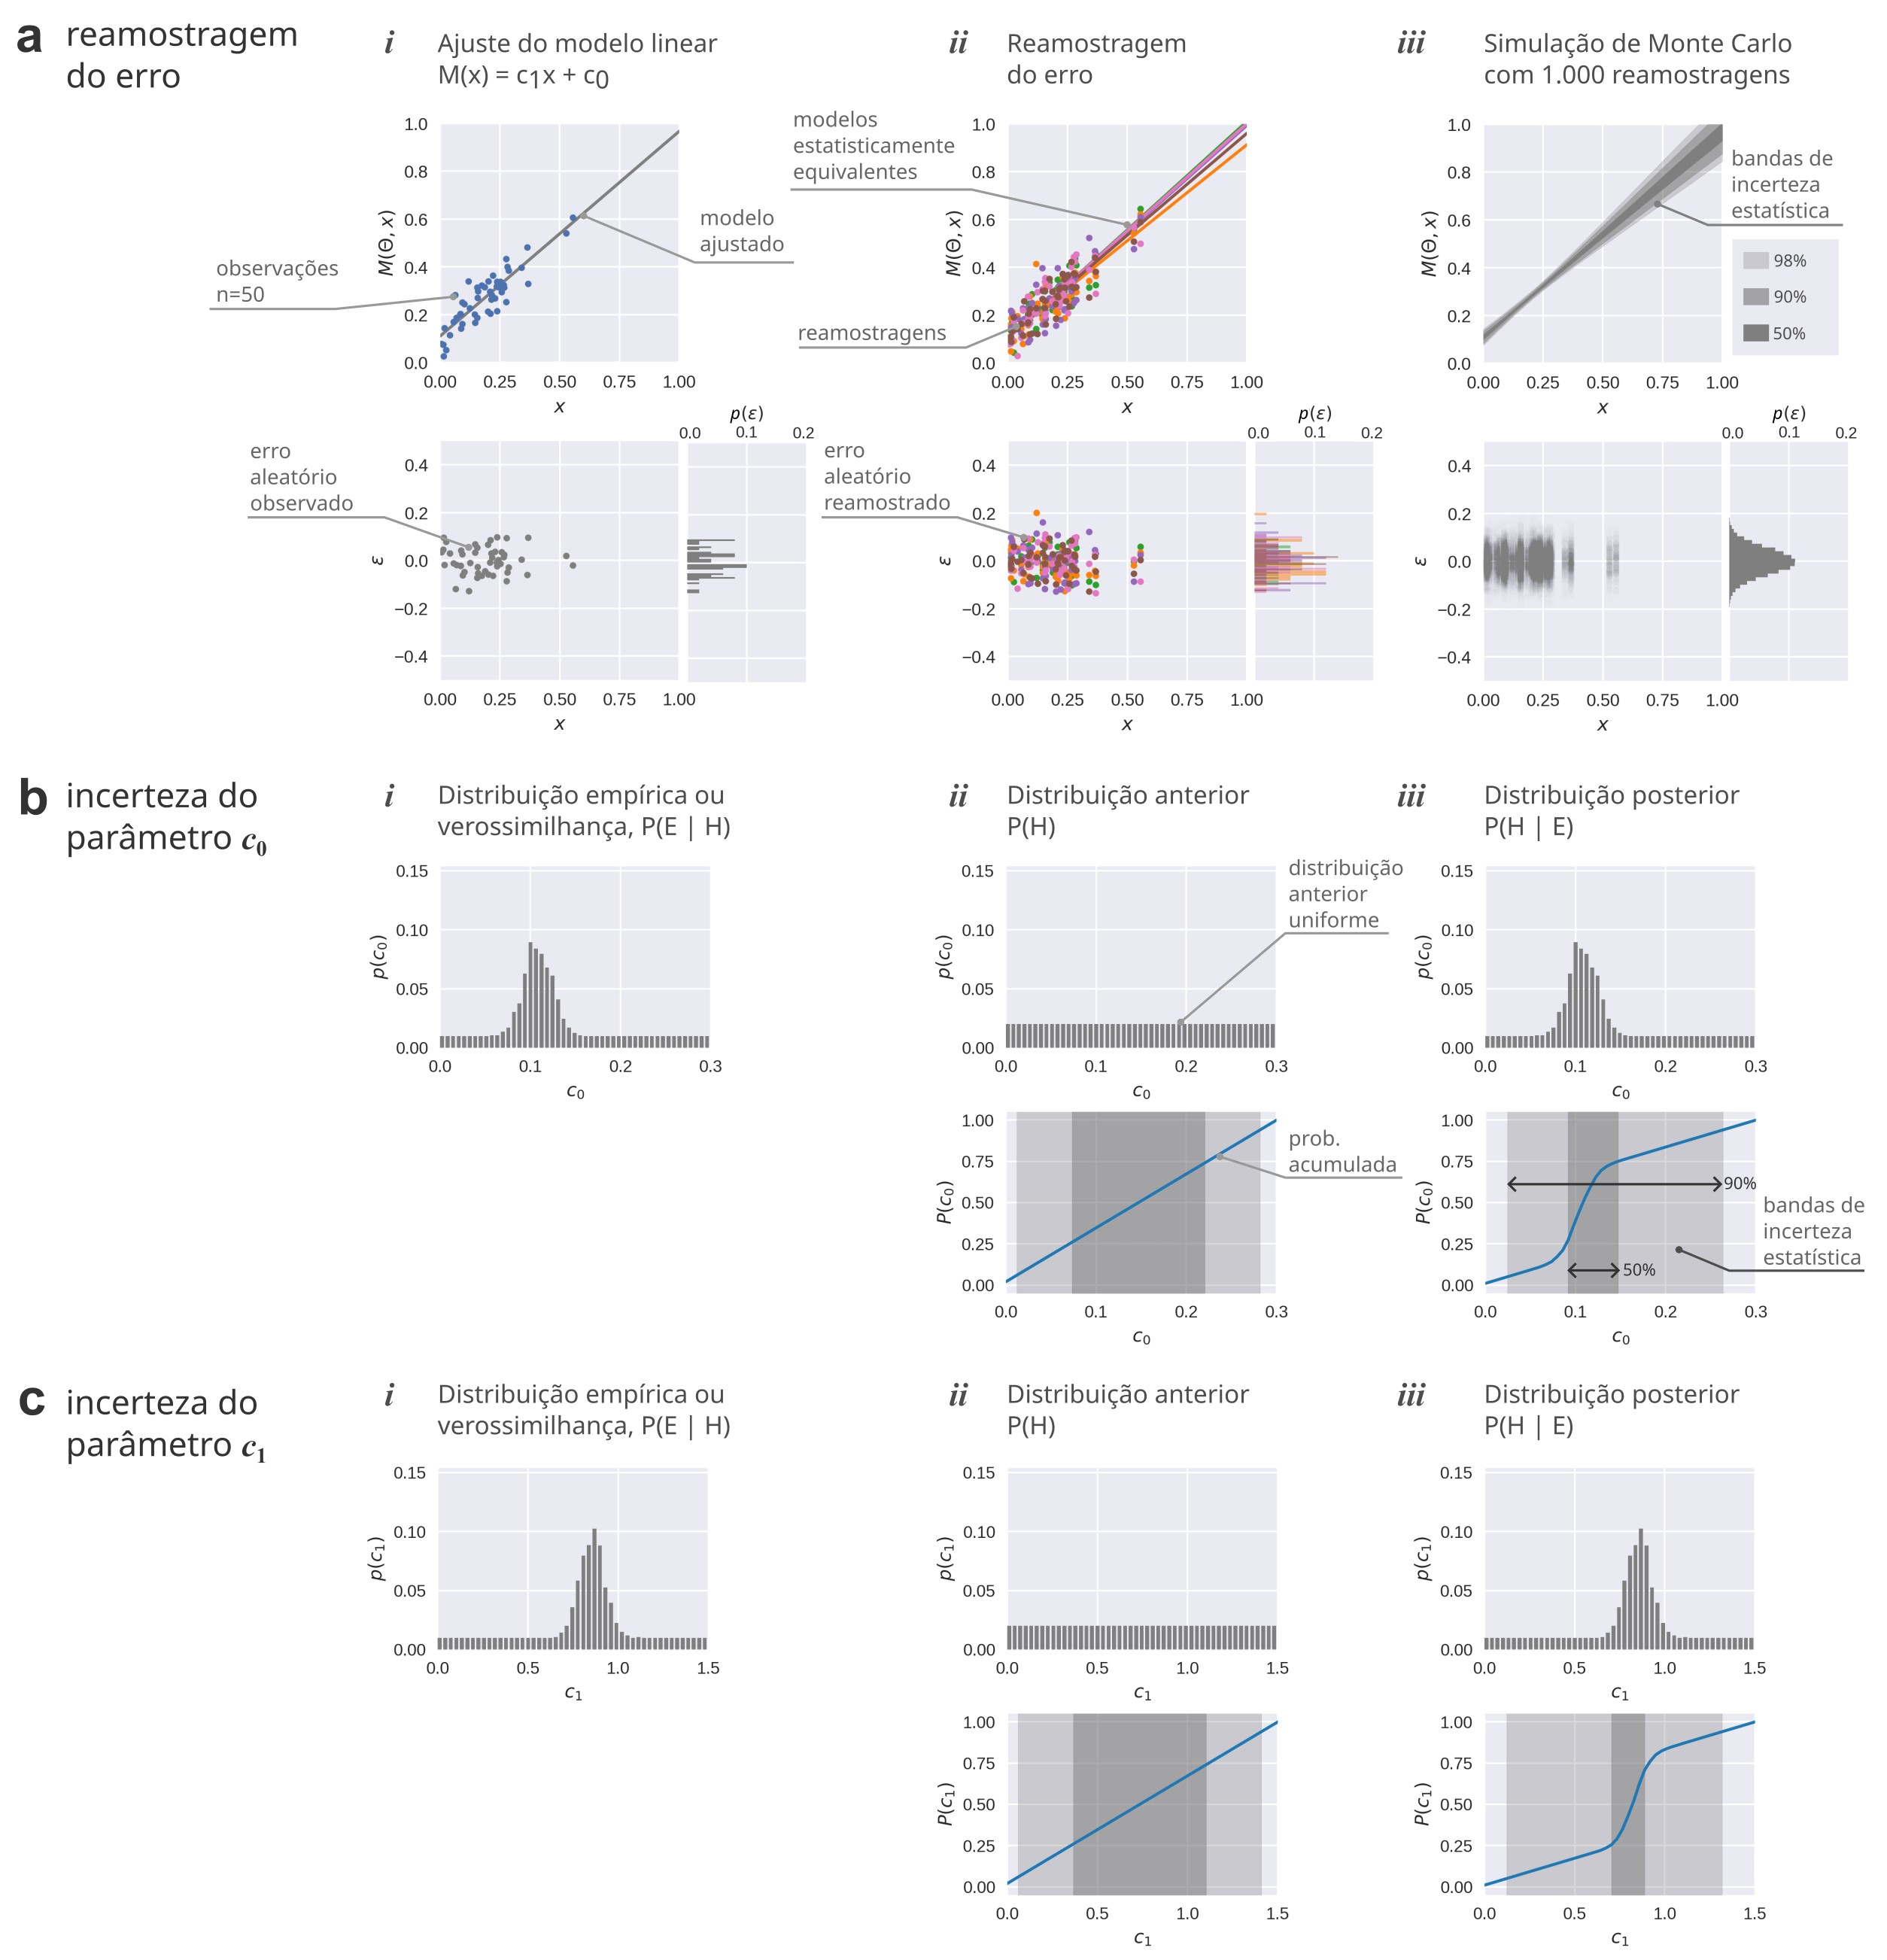
\includegraphics[width=0.95\linewidth]{fig_montecarlo_s1.jpg}		
	\caption[Primeira etapa de \gls{conditioning} de um \gls{model} linear]
	{\textbf{---\;Primeira etapa de \gls{conditioning} de um \gls{model} linear do tipo $M(x, \Theta) = c_{1}x + c_{0}$.}
        \;\textbf{a}\;---\;Ajuste de um \gls{model} linear pelo método dos mínimos quadrados. Esse primeiro ajuste permite que se estime o comportamento do erro $\varepsilon$ (detalhe a.\textit{\textrm{i}}.). Se as premissas sobre o erro forem atendidas, são realizadas inúmeras reamostragens do erro (\gls{monte-carlo}, detalhes a.\textit{\textrm{ii}}. e a.\textit{\textrm{iii}}). Para cada reamostragem, novos modelos são ajustados. O banco de dados das reamostragens permite a estimativa da distribuição de probabilidade empírica dos \gls{parameters} $c_0$ e $c_1$.\;\textbf{b}\;---\;Aplicação do Teorema de Bayes para se obter a distribuição posterior do parâmetro $c_0$ (detalhe b.\textit{\textrm{iii}}.). A distribuição empírica (detalhe b.\textit{\textrm{i}}.) foi obtida pelos resultados da simulação de Monte Carlo.\;\textbf{c}\;---\;Aplicação do Teorema de Bayes para se obter a distribuição posterior do parâmetro $c_1$ (detalhe c.\textit{\textrm{iii}}.). A distribuição empírica (detalhe c.\textit{\textrm{i}}.) foi obtida pelos resultados da simulação de Monte Carlo. Em ambos os casos a distribuição anterior foi considerada uniforme (b.\textit{\textrm{ii}}.; c.\textit{\textrm{ii}}.).
	}
\label{fig:bayes_s1}  % use qualitative label			
\end{figure}
% figure
\begin{figure}[t!] % place figure in the page
	\centering				
	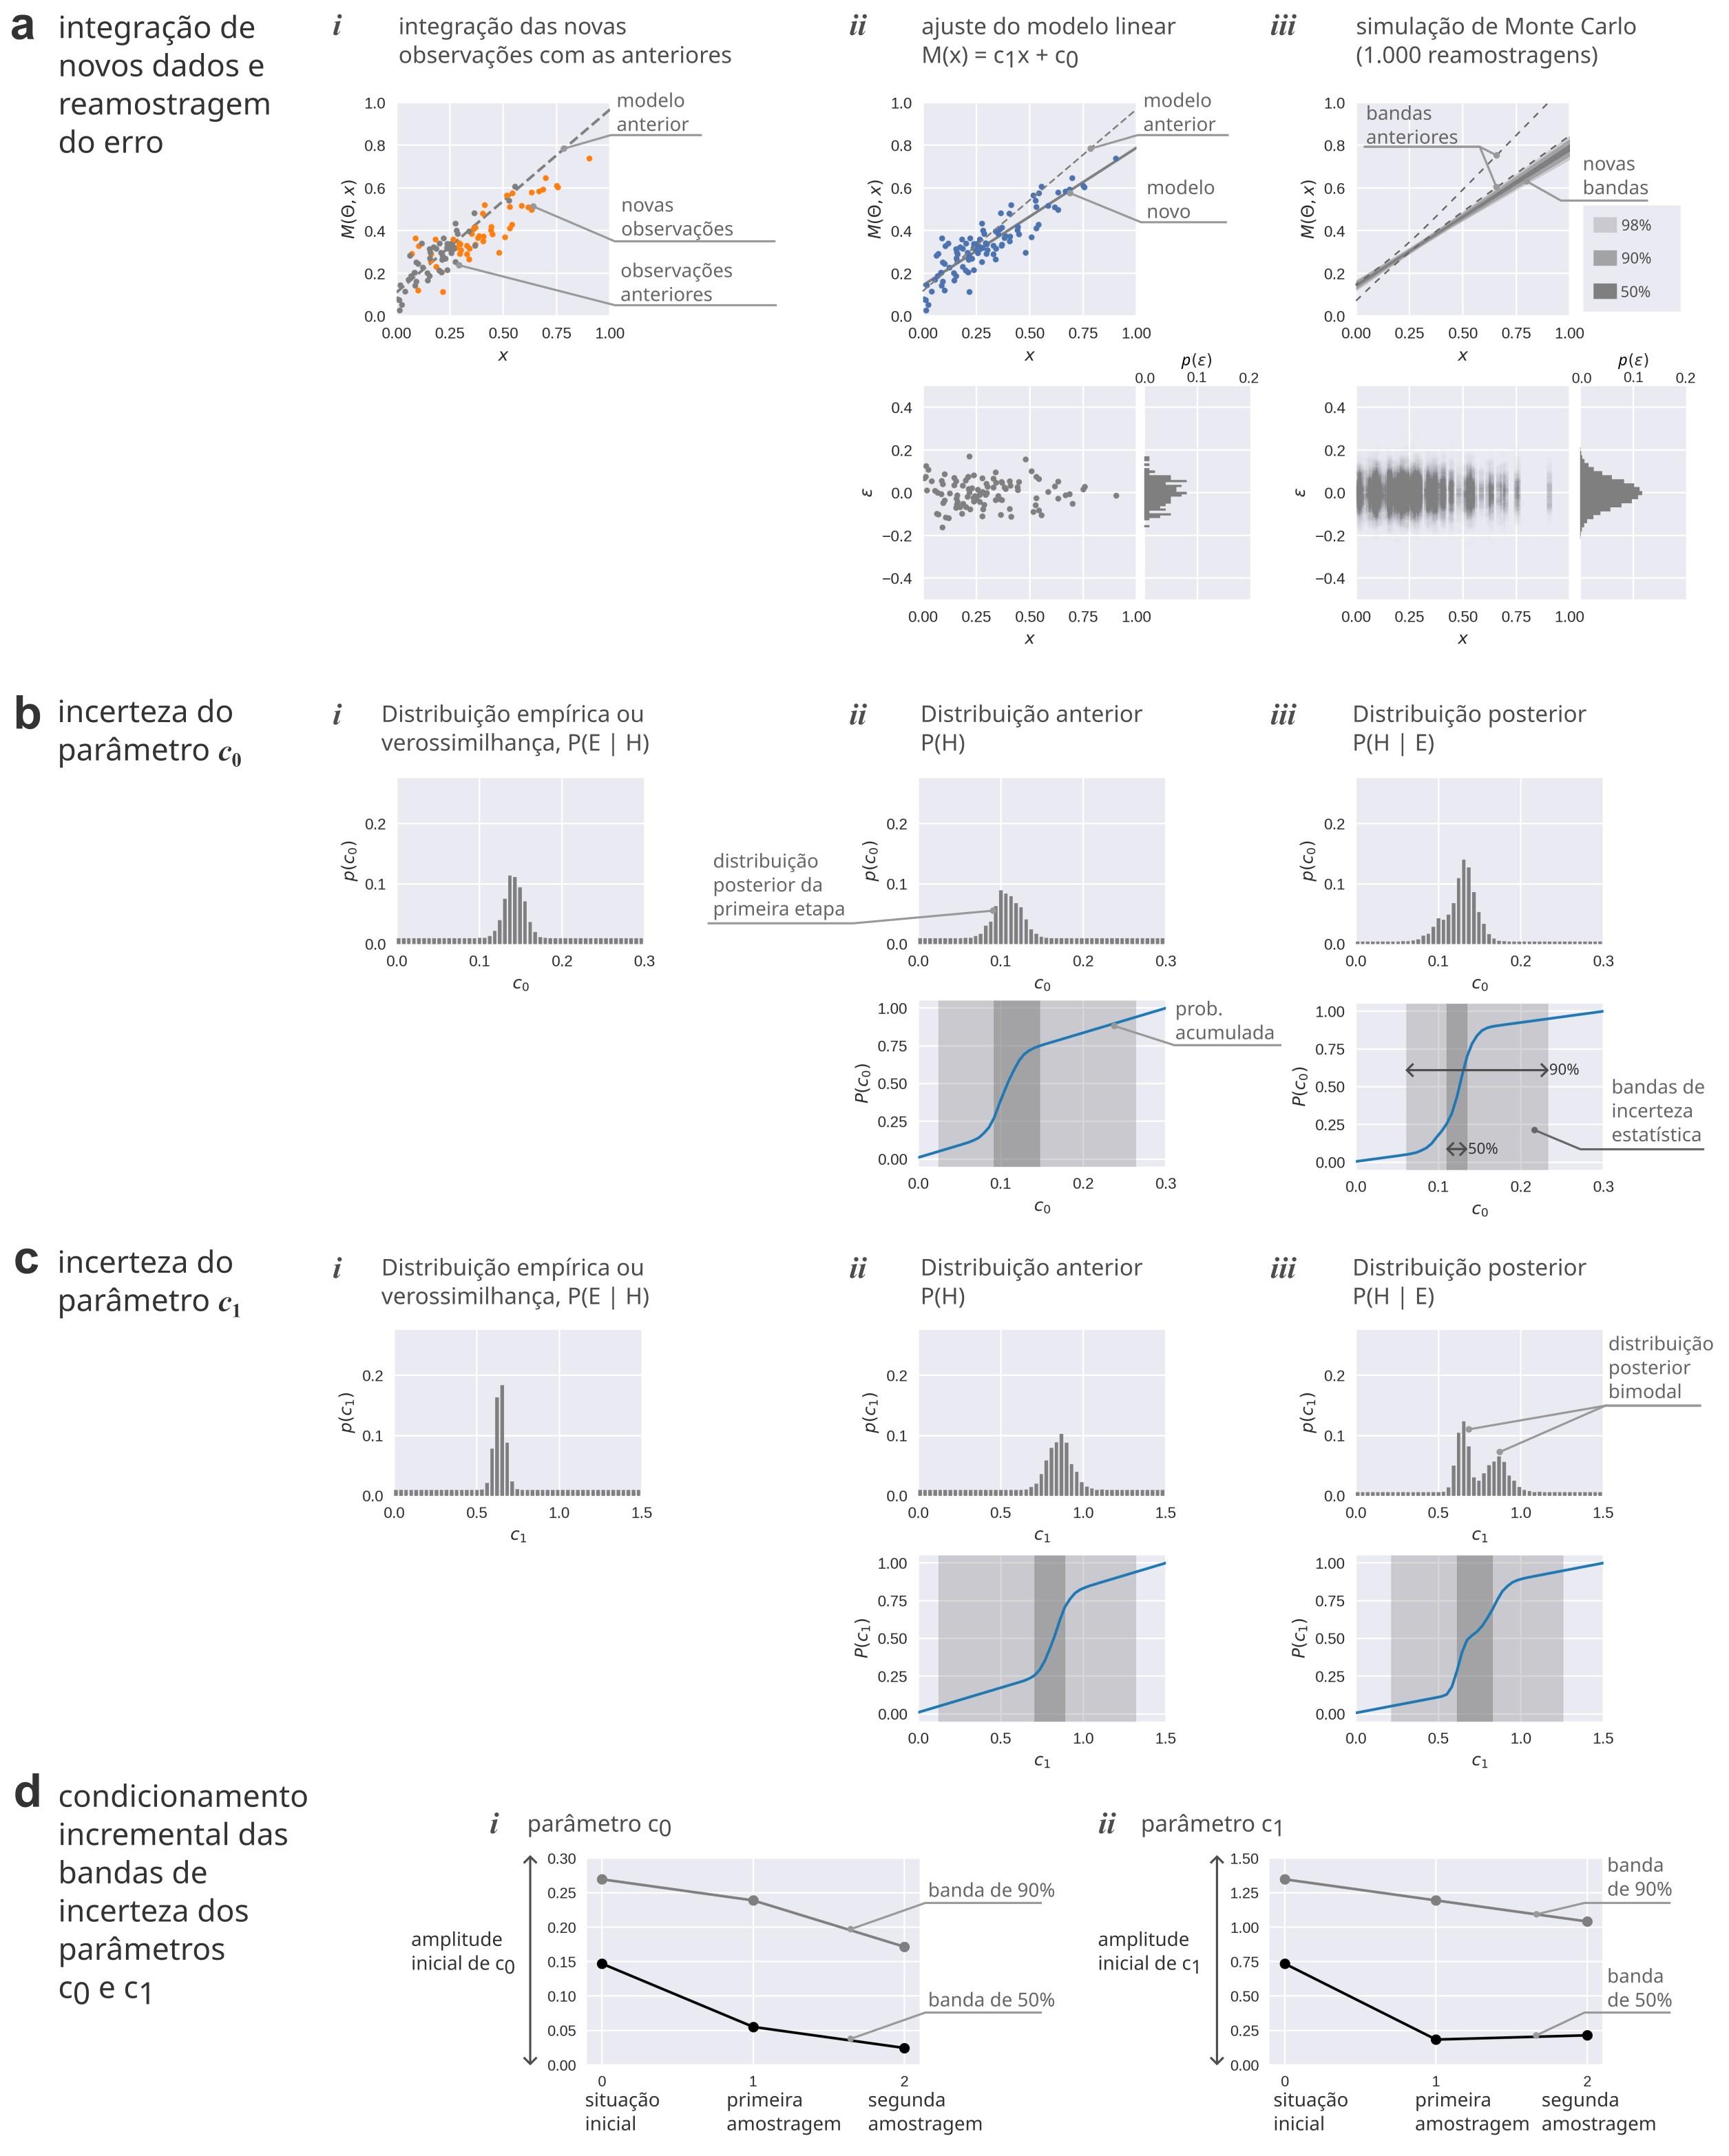
\includegraphics[width=0.95\linewidth]{fig_montecarlo_s2.jpg}		
	\caption[Segunda etapa de \gls{conditioning} de um \gls{model} linear]
	{\textbf{---\;Segunda etapa de \gls{conditioning} de um \gls{model} linear do tipo $M(x, \Theta) = c_{1}x + c_{0}$.}
        \;\textbf{a}\;---\;Segunda etapa de \gls{conditioning}. Os mesmos procedimentos são realizados como na primeira etapa, com a diferença que novos dados obtidos são integrados às observações anteriores e que a distribuição anterior utilizada é a distribuição posterior da primeira etapa.\;\textbf{b}\;---\;Aplicação do Teorema de Bayes para se obter a distribuição posterior do parâmetro $c_0$.\;\textbf{c}\;---\;Aplicação do Teorema de Bayes para se obter a distribuição posterior do parâmetro $c_1$.\;\textbf{d}\;---\;Análise das bandas de incerteza dos \gls{parameters} à medida que novas amostragens são feitas. As bandas de incerteza das predições e dos \gls{parameters} do \gls{model} foram reduzidas, com exceção da banda de incerteza de 50\% na segunda etapa do parâmetro $c_1$. Isso aconteceu porque as evidências na segunda amostragem são muito discordantes daquelas obtidas na primeira amostragem, resultando em uma distribuição posterior bimodal (detalhe c.\textit{\textrm{iii}}.).
	}
\label{fig:bayes_s2}  % use qualitative label			
\end{figure}
% figure
\begin{figure}[t!] % place figure in the page
	\centering				
	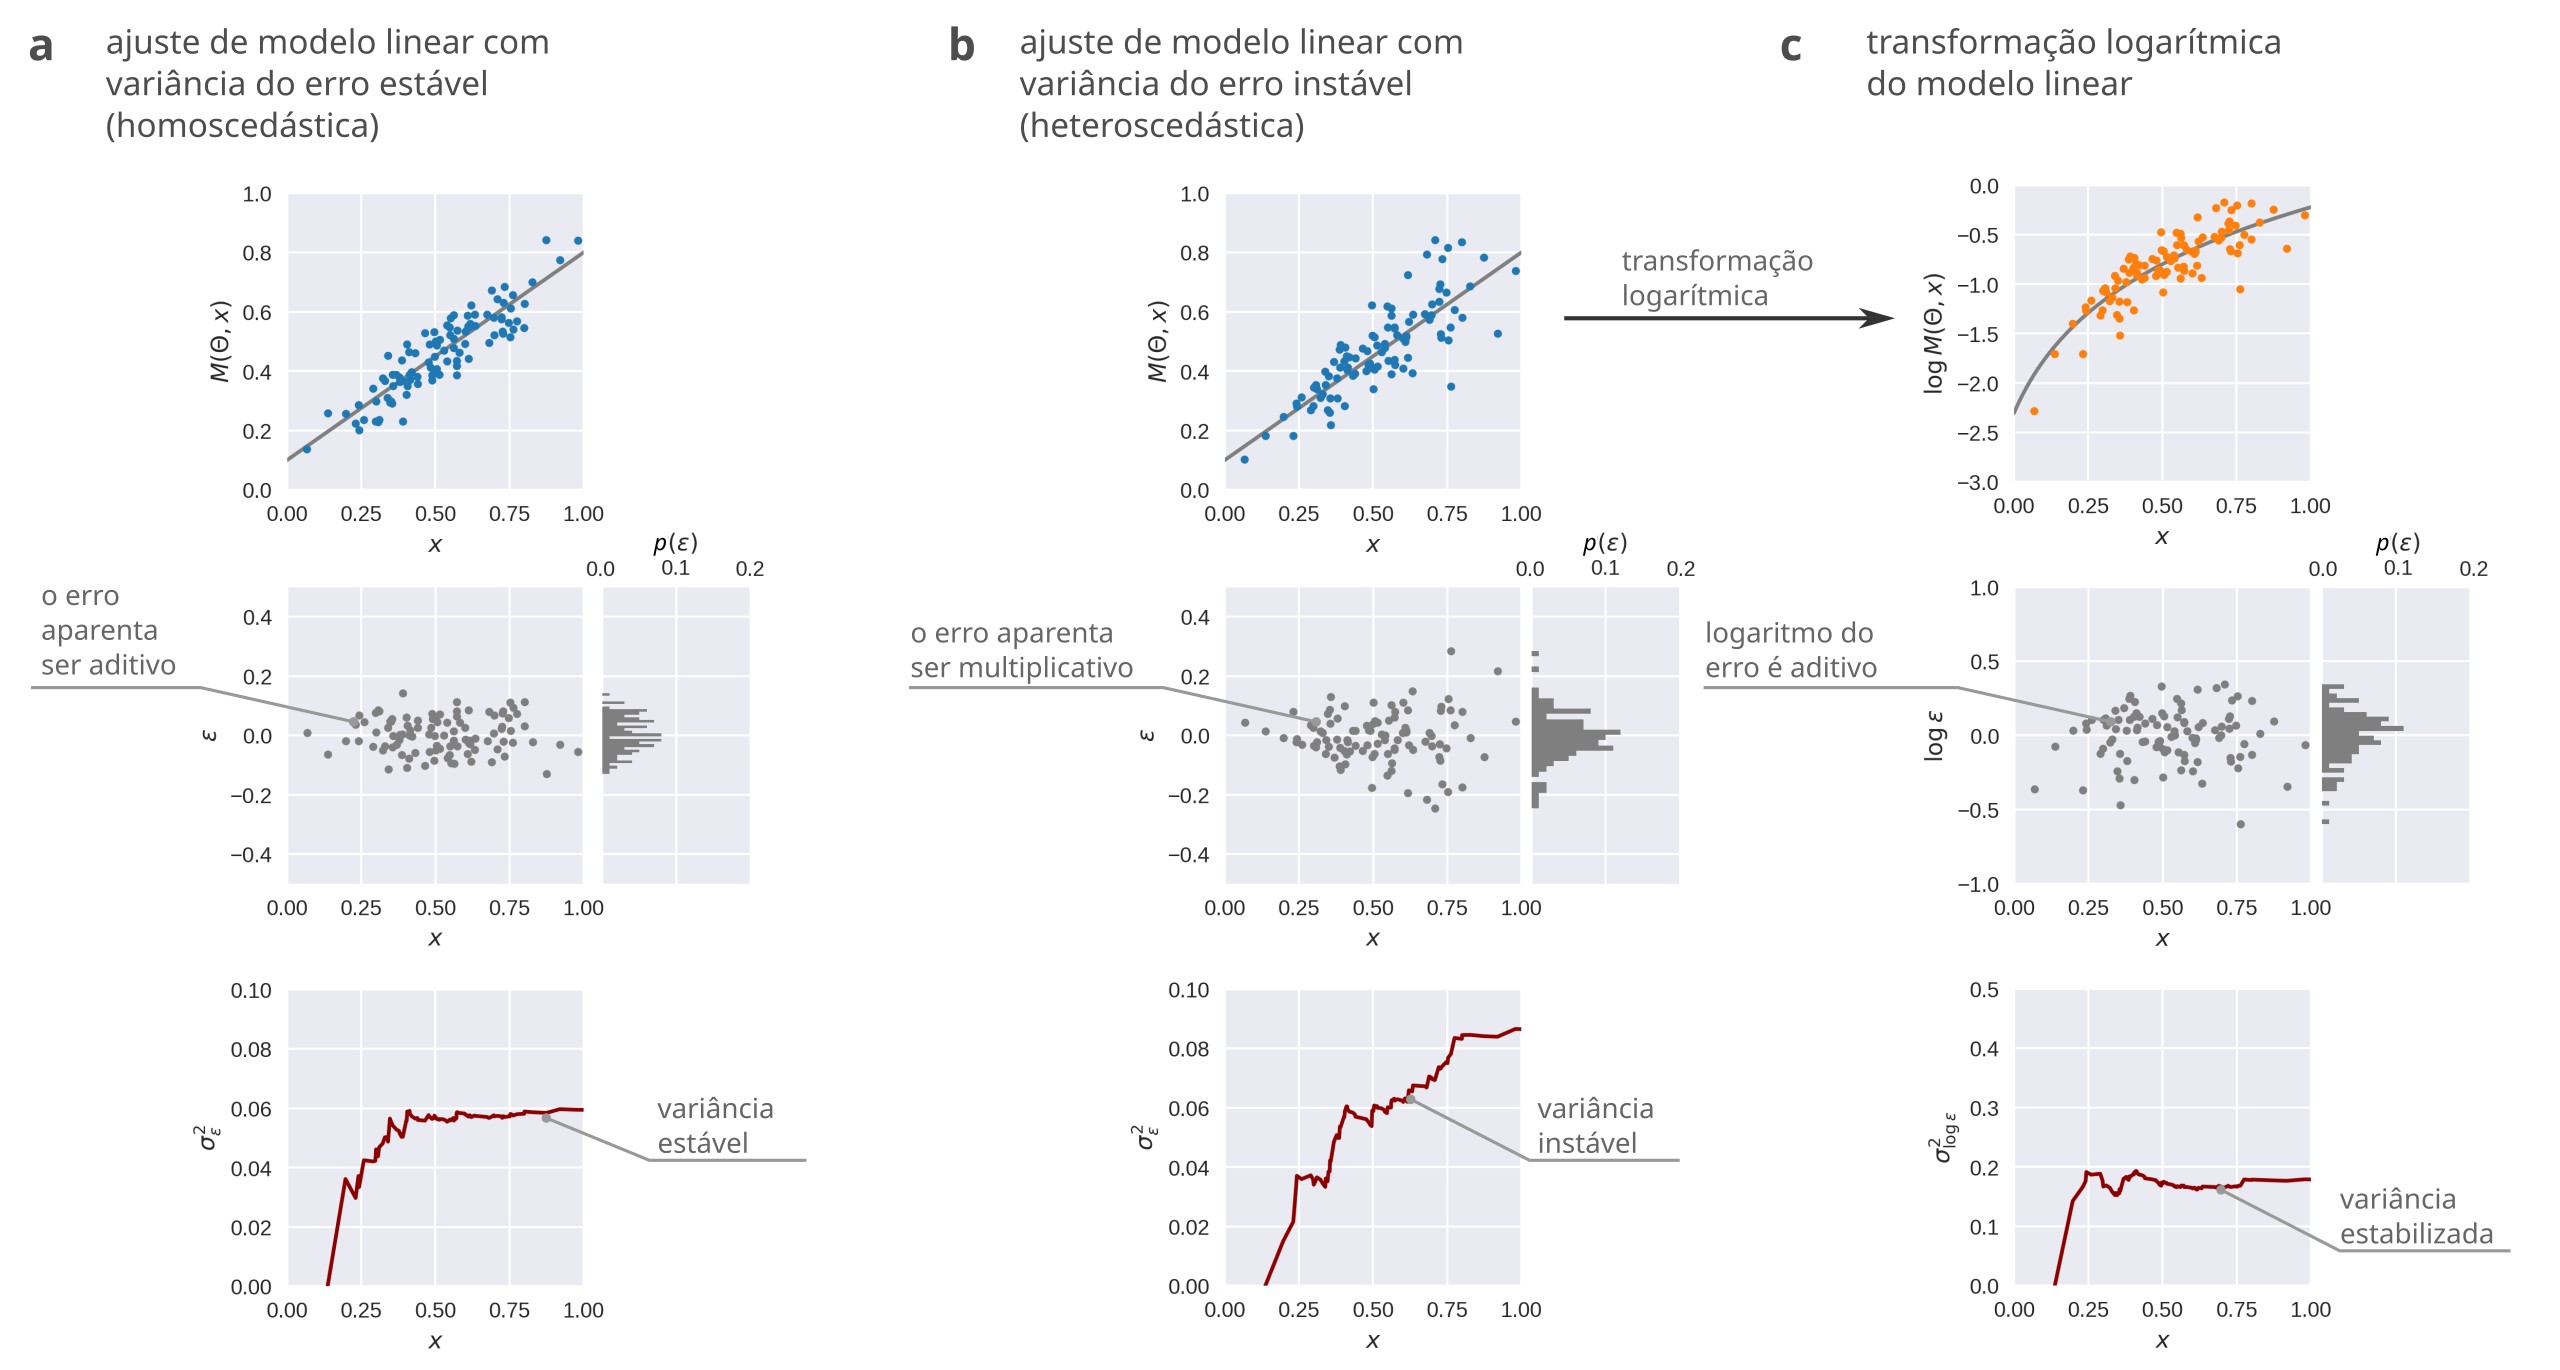
\includegraphics[width=0.95\linewidth]{fig_var_transform.jpg}		
	\caption[Erro aditivo e erro multiplicativo]
	{\textbf{---\;Erro aditivo e erro multiplicado no ajuste de um \gls{model} linear}
        \;\textbf{a}\;---\;Erro aditivo em um \gls{model} linear, com variância do erro estável (homoscedástica).\;\textbf{b}\;---\;Erro multiplicativo em um \gls{model} linear, com variância do erro instável (heterocedástica).\;\textbf{c}\;---\;Estabilização da variância do erro multiplicativo a partir de uma transformação logarítmica. O logaritmo do erro é aditivo.
	}
\label{fig:var_transform}  % use qualitative label			
\end{figure}
% sobre as ilustrações de simulação
\par A Figura \ref{fig:bayes_s1} e a Figura \ref{fig:bayes_s2} apresentam um exemplo ilustrativo para o processo de \gls{conditioning} de um \gls{model}. O objetivo foi condicionar um \gls{model} linear do tipo $M(x, \Theta) = c_{1}x + c_{0}$ pelas evidências empíricas disponíveis\footnote{Os dados aqui são sintéticos, gerados com o intuito de ilustrar a abordagem bayesiana.}. Note que $\Theta=\{c_{0}, c_{1}\}$, ou seja, o problema consiste obter a distribuição de \gls{posterior} dos \gls{parameters} $c_0$ e $c_1$. Vejamos primeiramente o caso da situação inicial (Figura \ref{fig:bayes_s1}), quando a primeira amostra de dados empíricos foram obtidos ($n=50$). Diante dos dados, o \gls{model} $M(x, \Theta)$ foi ajustado pelo métodos dos mínimos quadrados. O valor exato obtido para os \gls{parameters} no ajuste inicial é \textbf{irrelevante}, pois estamos interessados em obter uma distribuição de probabilidade, não valores precisos. O ajuste inicial do \gls{model} tem a única função de produzir uma estimativa da dispersão do erro $\varepsilon$. Por simples inspeção visual, percebe-se que a distribuição dos erros do \gls{model} ajustado apresenta uma boa simetria em torno do zero e uma dispersão estável. Assumindo-se então que o erro $\varepsilon$ apresenta distribuição normal com média zero e variância constante, o método de Monte Carlo foi aplicado para mil reamostragens, que foram feitas aproximando-se a variância populacional pela variância amostral (isto é, $\sigma^2_\varepsilon \approx s^2_\varepsilon$). Em cada simulação, novos ajustes para o \gls{model} foram feitos, de maneira que foi possível se estimar as bandas de incerteza para o \gls{model} $M(x, \Theta)$.  Por fim, a distribuição da \gls{likelihood} $P(E | H)$ dos \gls{parameters} $c_0$ e $c_1$ foi estimada a partir do histograma da lista de mil valores estatisticamente equivalentes gerados pelas simulações. Como a distribuição anterior $P(H)$ era uniforme, o padrão da distribuição posterior $P(H | E)$ foi completamente influenciado pela \gls{likelihood}. Agora vejamos a segunda etapa (Figura \ref{fig:bayes_s2}), quando uma nova amostra de dados empíricos foi inserida ($n=50$). Nessa etapa, os novos dados foram misturados aos antigos e se procedeu da mesma forma que antes: um \gls{model} foi ajustado aos dados e novas simulações do erro $\varepsilon$ foram feitas aproximando-se a sua variância populacional pela sua variância amostral. A exceção consistiu no fato de que a distribuição anterior agora é justamente a distribuição posterior obtida na situação inicial. Com isso, o advento de novas observações empíricas podem tanto \textit{reforçar} quanto \textit{atenuar} o \gls{grau-convic} obtido anteriormente para os \gls{parameters} $c_0$ e $c_1$. No caso ilustrado, é evidente que as novas observações atenuaram suavemente o \gls{grau-convic} no caso do parâmetro $c_1$, alargando um pouco a banda de incerteza de 50\% obtidas na primeira etapa e gerando uma distribuição posterior bimodal. 

\par Na Equação \eqref{eq:bayes-model} está embutida a premissa de que o erro $\varepsilon$ é \textit{linearmente aditivo} ao \gls{model}. Mas ele poderia ser \textit{multiplicativo}, o que faria a Equação \eqref{eq:bayes-model} assumir a seguinte forma:
\begin{linenomath*}
\begin{equation}
\label{eq:bayes-model-multi}
    O(x, t) = M(x, t, \Theta) \cdot \varepsilon(x, t)
\end{equation}
\end{linenomath*}
Essa premissa faz sentido quando o ruído aleatório é cada vez maior à medida que a variável independente cresce. No caso das curvas-chave, é razoável esperar que erros proporcionalmente maiores estejam presentes na medição de vazões altas a partir do nível d'água, principalmente (mas não somente) em razão das maiores incertezas na geometria e rugosidade da seção do canal. Quando isso ocorre, a variância do erro não é constante, mas aumenta gradativamente. Nesse caso, a variância é heteroscedástica (instável), ao contrário de homoscedástica (estável). Uma alternativa para abordar esse caso é através da \textbf{transformação de variáveis}, convertendo o problema para um caso aditivo ao se tomar o logaritmo em ambos os lados da Equação \eqref{eq:bayes-model-multi}, pois $\log(ab) = \log(a) + \log(b)$. Com isso, as premissas  mencionadas anteriormente podem ser avaliadas sobre $\log(\varepsilon)$, que possivelmente apresenta variância estável. Para aplicar o método de Monte Carlo, as reamostragens do erro podem ser feitas diretamente em $\log(\varepsilon)$ e convertidas de volta na Equação \eqref{eq:bayes-model-multi} para o ajuste do \gls{model} $M(x, \Theta)$ por técnicas de otimização. A Figura \ref{fig:var_transform} ilustra esse processo.

\begin{simplebox}[
    float=htb,
    label={destaque_curvas_chave},
    nameref={Curvas-chave}
    ]{Bandas de incerteza de vazão a partir de curvas-chave}
    \footnotesize
    % first minipage
    \begin{minipage}[t]{\linewidth}    
    \par A \textbf{vazão} em rios quase nunca é medida diretamente, pois para isso é preciso uma equipe técnica especializada. É muito mais fácil e barato observar o \textbf{nível} dos rios a partir de réguas linimétricas. De fato, o nível de muitos rios no Brasil é observado duas vezes ao dia em estações fluviométricas da Rede Hidrometeorológica Nacional. Assim, as raras observações de vazão factíveis são utilizadas na construção de uma \textbf{curva-chave}, que geralmente é um \gls{model} matemático do tipo potência:
    \begin{equation*} % the equation environment. 
    		\label{eq:rating_curve}
    		Q = a \cdot (h - h_0)^b
    \end{equation*}
    Em que $Q$ é a vazão em $m^{3}/s$; $h$ é o nível observado, e; $h_0$, $a$ e $b$ são os \gls{parameters} do \gls{model}. Essa curva pode então ser usada para a estimativa da vazão a partir das observações rotineiras de nível. 
    \end{minipage}
    % second min
    \begin{minipage}[t]{\linewidth}
        \begin{minipage}[t]{\linewidth}
        \vspace*{5pt}
        	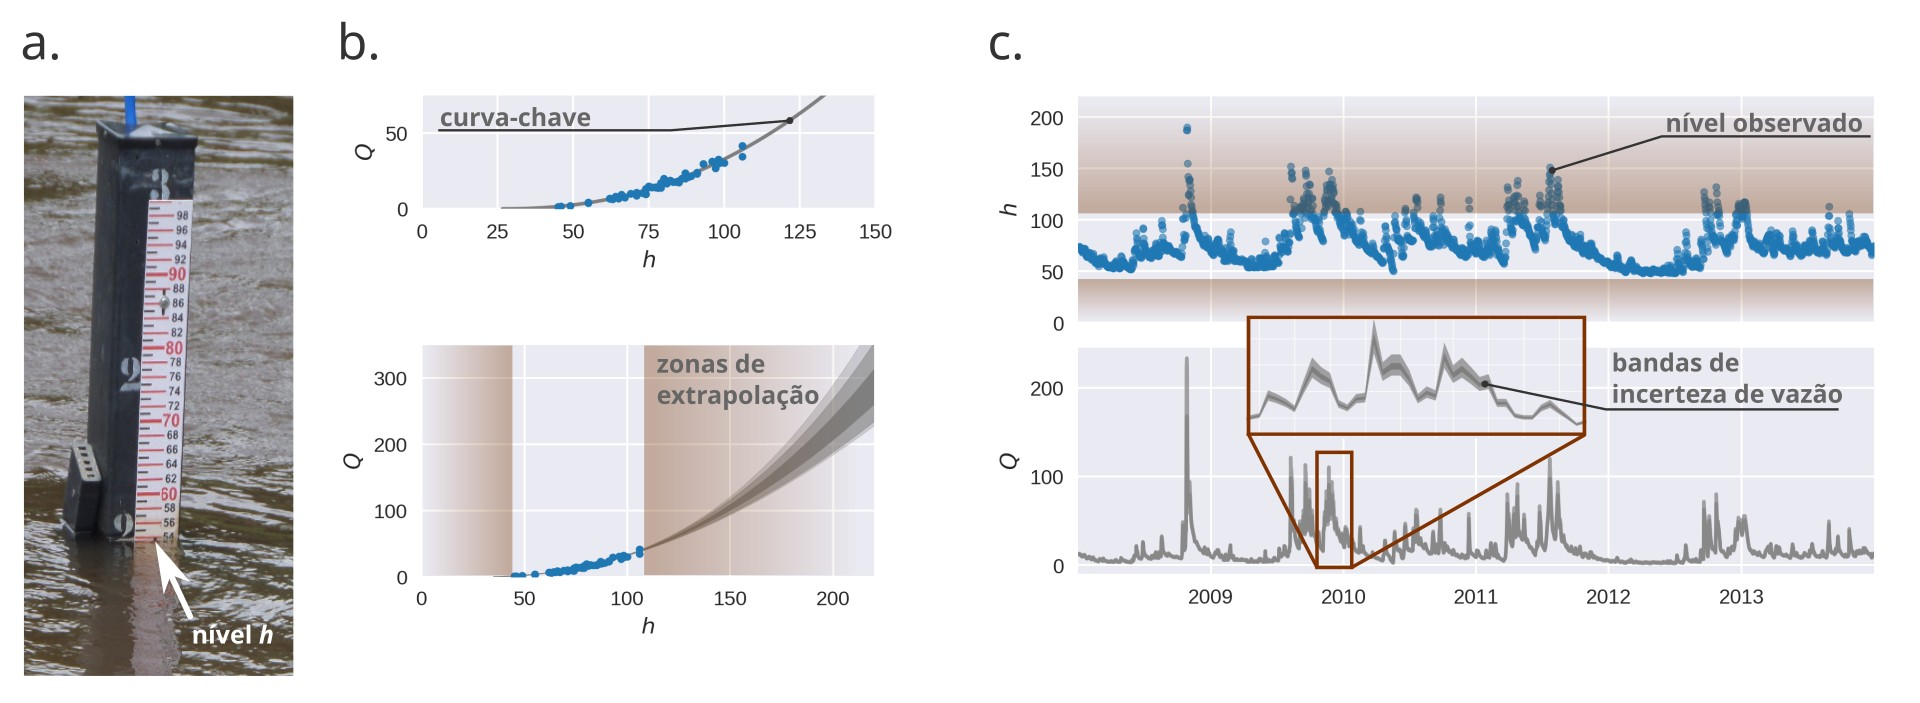
\includegraphics[width=\linewidth]{fig_ratingcurve.jpg}		
        	\captionof{figure}[Bandas de incerteza de vazão a partir de curvas-chave]{
                \textbf{---\;Bandas de incerteza de vazão a partir de curvas-chave.}\;\textbf{a}\;---\;Observação de nível $h$ em uma régua linimétrica.\;\textbf{b}\;---\;Ajuste de um \gls{model} tipo potência e estimativa da incerteza por métodos de reamostragem do erro.\;\textbf{c}\;---\;Série histórica de nível e bandas de incerteza da vazão.
        	}
            \label{fig:rating-curve}  % use qualitative label	
        \vspace*{5pt}
    \end{minipage}
    % next
    \end{minipage}
    \begin{minipage}[t]{\linewidth}
    \par Como ilustrado na Figura \ref{fig:rating-curve}, a confirmação desse \gls{model} diante das evidências de nível e vazão inicia-se por ajustar os \gls{parameters} aos dados disponíveis com técnicas de otimização. O comportamento do erro aleatório pode ser então avaliado. A variância do erro, se estabilizada, permite reamostragens estatisticamente equivalentes dos dados (simulações de Monte Carlo). As bandas de incerteza da \gls{rating-curve}, assim, se refletem na incerteza da estimativa na série histórica de vazão. No exemplo apresentado, nota-se que existem \textbf{zonas de extrapolação} nos extremos, onde a incerteza se expande desproporcionalmente. Isso é esperado, pois eventos extremos de vazão são raros ou difíceis de serem medidos. Por outro lado, a captura de poucos eventos extremos pode reduzir drasticamente a incerteza nessas zonas. 
    \par Uma abordagem interessante nesse contexto é apresentada por Thomas Morlot e colegas, que salientam que além das incertezas estatísticas, as curvas-chave apresentam uma dependência temporal associada à mudança na morfologia da seção do rio \cite{Morlot2014}. Outras complexidades também existem, como a histerese hidráulica que pode se manifestar sob diferentes regimes de escoamento.    
    \end{minipage}
\label{box:rating-curve}
\normalsize
\end{simplebox}

\section{Rejeição} \label{sec:epis:popper}

\par Apesar do sucesso do \gls{empiricism} como corrente hegemônica na Filosofia da Ciência na modernidade, as mudanças impressionantes na Física no século XX deram mais uma chance ao \gls{rationalism}, ou seja, para a abordagem dedutiva em relação ao \gls{problem-just}. O impacto da obra de Albert Einstein (1879-1955) é um bom exemplo desse momento histórico. No caso, Einstein revolucionou a Física a partir do que ele chamava de \textit{experimentos mentais}. Se teorias são produto da experiência empírica, como clamam os empiristas, Einstein jamais teria escrito seus primeiros artigos, pois na época trabalhava em uma empresa de patentes e não tinha acesso a laboratórios ou outros recursos para coletar dados empíricos. Ao contrário, foram outros cientistas que, com observações e experimentos, deram suporte para a \gls{teoria} de Einstein \textit{a posteriori}, ou seja, \textit{depois} que as suas ideias já estavam publicadas. Algo estava definitivamente errado na corrente empirista de justificação de teorias.

\par O expoente desse novo movimento racionalista foi o filósofo Karl Popper (1902-1994), especialmente com sua obra \textit{A lógica da pesquisa científica}. Ele introduziu a corrente hoje denominada de \textbf{\gls{critical-rationalism}}, também chamada de \textbf{abordagem hipotético-dedutiva} \sethlcolor{cyan}\hl{[todo:cite]}. Por um lado, Popper estava ciente da gravidade do \gls{problem-indu}, que permaneceu (e permanece) sem solução desde sua formulação por Hume – para ele, o \gls{empiricism} indutivista claramente não poderia se sustentar. Por outro, as correntes filosóficas de sua época ditas Convencionalistas também não o agradavam, ainda que representassem abordagem dedutivas para a justificação de teorias. Nesse sentido, Popper concluiu que o grande poder epistêmico das evidências empíricas é justificar, pelo método dedutivo, a \textit{falsidade} de uma \gls{teoria}. Ou seja, é pela \textbf{rejeição}\footnote{Aqui o termo \textit{rejeição}, \textit{refutação} e \textit{falsificação} são usados de forma equivalente.} de teorias pelas evidências que o conhecimento verdadeiro é obtido.

\par Um exemplo simples transmite a força desse argumento. 

\par Considere o enunciado universal de que \say{\textit{todos os cisnes são brancos}}. Para estabelecer definitivamente a verdade desse enunciado pelo método indutivo, seria preciso observar todos os cisnes que existem no universo, inclusive cisnes no passado e no futuro, o que é obviamente impossível na prática. Por outro lado, só é preciso avistar um \textit{único cisne preto} (ou de qualquer outra cor) no tempo e no espaço para refutar definitivamente a \gls{teoria} de que todos os cisnes são brancos. Afinal, se o enunciado singular \say{\textit{um certo cisne é preto}} é verdadeiro (pois foi verificado empiricamente), então deduzimos que o enunciado universal \say{\textit{todos os cisnes são brancos}} é falso:
\begin{linenomath*}
    \begin{align*}
        S_1 \implies S_2 & \quad \textnormal{se todos os cisnes são brancos, então um certo cisne é branco} \\
        \neg S_2 & \quad \textnormal{um certo cisne \textbf{não} é branco}\\
        \therefore\;\neg S_1 & \quad \textnormal{portanto, nem todos os cisnes são brancos}
    \end{align*}
\end{linenomath*}
Esse modo de lógica dedutiva, por envolver a negação, chama-se \textit{modus tollens}, ao contrário do \textit{modus ponens}, que envolve a afirmação positiva. O que Popper demonstra é que existe uma assimetria fundamental entre esses dois modos de lógica quando queremos deduzir enunciados universais a partir de enunciado singulares (fazer generalizações a partir de observações pontuais), sendo o \textit{modus tollens} a única forma de se obter conhecimento seguro (no caso, a falsidade de um enunciado universal). Daí decorre que as observações e experiências empíricas são importantes para refutar teorias, não para confirmá-las. Enquanto uma \gls{teoria} sobrevive a rigorosos testes empíricos, se diz que essa \gls{teoria} é \textit{corroborada} pelas evidências empíricas – mas nunca confirmada.

\par Alicerçado com esse argumento, Popper se volta para o que ele chama de \textbf{\gls{problem-demarc}}, trazido inicialmente por Kant: a dificuldade de distinguir se uma \gls{teoria} é \textit{científica} ou é \textit{apenas metafísica}, baseada unicamente em abstrações. Ao contrário dos empiristas, que alegam que a experiência é a origem de todo o conhecimento, para Popper a origem de onde as teorias surgem é irrelevante. Desde que sejam logicamente consistentes, elas podem se manifestar tanto a partir de alguma observação empírica motivadora (como no exemplo dos cisnes brancos), quanto a partir da intuição criativa (como os experimentos mentais feitos por Einstein). O que é relevante é a capacidade da \gls{teoria} não sobreviver aos testes da experiência empírica, ou seja, a capacidade de ser rejeitada. Essa capacidade, que se denomina \textbf{\gls{falseabilidade}}, é o \textit{critério de demarcação} que categoriza uma \gls{teoria} como científica. Resumidamente, na ótica do \gls{critical-rationalism}, uma \gls{teoria} científica deve ser falseável. Aqui, é importante frisar que \textit{ser falseável }não quer dizer \textit{ser falsa}. Ser falseável significa que a estrutura da \gls{teoria} autoriza que observações possam ser usadas para demonstrar a sua eventual falsidade. Se \textit{por princípio} é impossível provar que uma \gls{teoria} é falsa a partir de observações ou experimentos, então essa \gls{teoria} não é científica. Isso geralmente implica que teorias científicas devem ser precisas o suficiente para produzirem predições observáveis. No caso de Einstein, sua \gls{teoria} era precisa e fazia predições observáveis que foram, no jargão de Popper, \textit{corroboradas} por outros cientistas (mas que poderiam ter sido perfeitamente refutadas). Já um exemplo intuitivo de \gls{teoria} não falseável é a \gls{teoria} do Multiverso, uma \gls{teoria} cosmológica que postula a existência de Universos paralelos ao que habitamos. Por mais sedutora que seja para \textit{explicar} alguns mistérios cosmológicos, essa \gls{teoria} não é científica pois não autoriza nenhum \textit{teste} com observações empíricas – por princípio, não há como observar além de nosso próprio Universo. Nas palavras de Popper: 

\begin{adjustwidth}{100pt}{0pt}
\medskip
\small (...) uma \gls{teoria} é algo que o entendimento tenta prescrever à natureza; algo que a natureza frequentemente não permite que se prescreva a ela; uma \gls{hipotese} que nós tentamos impor à natureza, mas que pode ser desmentida por ela -- Karl Popper \cite{popper2013dois}.
\medskip
\end{adjustwidth}

\par Uma vez designada a \gls{falseabilidade} como critério de demarcação de teorias científicas, Popper avança para o então chamado \textbf{problema da simplicidade}. Esse problema epistemológico consiste na dificuldade de explicar por que se deve preferir teorias mais simples do que teorias mais complexas (também conhecido por \textit{navalha de Occam}). Por exemplo, considere uma série de observações pontuais de um dado fenômeno dispostas em um \gls{system} de coordenadas. Se existe uma lei teórica que descreve esse fenômeno, essa lei será uma curva que liga todos os pontos observados. Só que para um número finito de pontos sempre é possível ajustar um número infinito de curvas com as mais diversas fórmulas matemáticas. Se uma reta apresentar um bom ajuste, isso também é possível com a parte assintótica de uma hipérbole. Como vimos na seção anterior, ainda que os empiristas bayesianos possuem métodos para atualizar o \gls{grau-convic} no ajuste de uma dada curva à medida que novas observações são coletadas, eles não têm nada a dizer sobre a justificativa de ter \textit{escolhido essa curva em primeiro lugar}, a não ser a sua suposta \textit{simplicidade}. Esse é de fato um problema confuso, pois depende do que queremos dizer com o conceito de simplicidade. Para uns, significa um aspecto estético, algo relacionado à elegância matemática – como o fato de órbitas circulares para os planetas parecerem mais bonitas que órbitas elípticas. Para outros, quer dizer um aspecto pragmático, algo relacionado à economia de tempo e recursos – um método mais fácil para resolver uma tarefa deve ser preferido do que um método mais intrincado. O estatístico George Box (1919-2013), por exemplo, defende o que ele chama de \textbf{princípio da parcimônia} em modelos matemáticos por critérios puramente práticos, como a carga cognitiva, melhor precisão e objetividade \cite{Box1979}.

\par Em vista disso, Popper elimina qualquer caráter estético ou pragmático, igualando a simplicidade de uma \gls{teoria} com o seu \textbf{grau de falseabilidade}: quanto mais simples, mais falseável. Isso resolve logicamente o problema da simplicidade, pois, nas suas palavras:

\begin{adjustwidth}{100pt}{0pt}
\medskip
\small Os enunciados simples (...) nos dizem mais, porque encerram um conteúdo empírico maior e porque são suscetíveis de testes mais rigorosos -- Karl Popper \cite{popper2004logica}.
\medskip
\end{adjustwidth}

\noindent Ou seja, enquanto uma \gls{teoria} mais simples, que é mais \textit{restritiva}, sobreviver aos testes empíricos, não faz sentido lógico adotar uma \gls{teoria} menos simples, que é mais \textit{flexível}. Isso fica mais claro em termos matemáticos, pois o número de \gls{parameters} de uma curva está inversamente associado ao seu grau de \gls{falseabilidade}. Considere uma curva com três \gls{parameters}, como um polinômio de segundo grau (uma parábola): $f(x) = c_{2}x^{2} + c_{1}x + c_{0}$. Essa curva é muito mais flexível para ajustar dados que uma curva com dois \gls{parameters}, como um polinômio de primeiro grau (uma reta): $g(x) = c_{1}x + c_{0}$. Afinal, se fizermos o parâmetro quadrático $c_{2}$ suficientemente pequeno, podemos ajustar igualmente bem os dados de uma linha reta $g(x)$ sem falsear a \gls{teoria} que o fenômeno estudado é descrito pela parábola $f(x)$, pois $\lim_{c_{2}\to0} f(x) = g(x)$. A mesma lógica se aplica para órbitas circulares e elípticas: a \gls{teoria} do círculo, sendo essa curva um caso específico de elipse, deve ser preterida antes da \gls{teoria} da elipse não por sua estética, mas por sua facilidade de ser demonstrada falsa pelas evidências observadas.
% figure
\begin{figure}[t!] % place figure in the page
	\centering				
	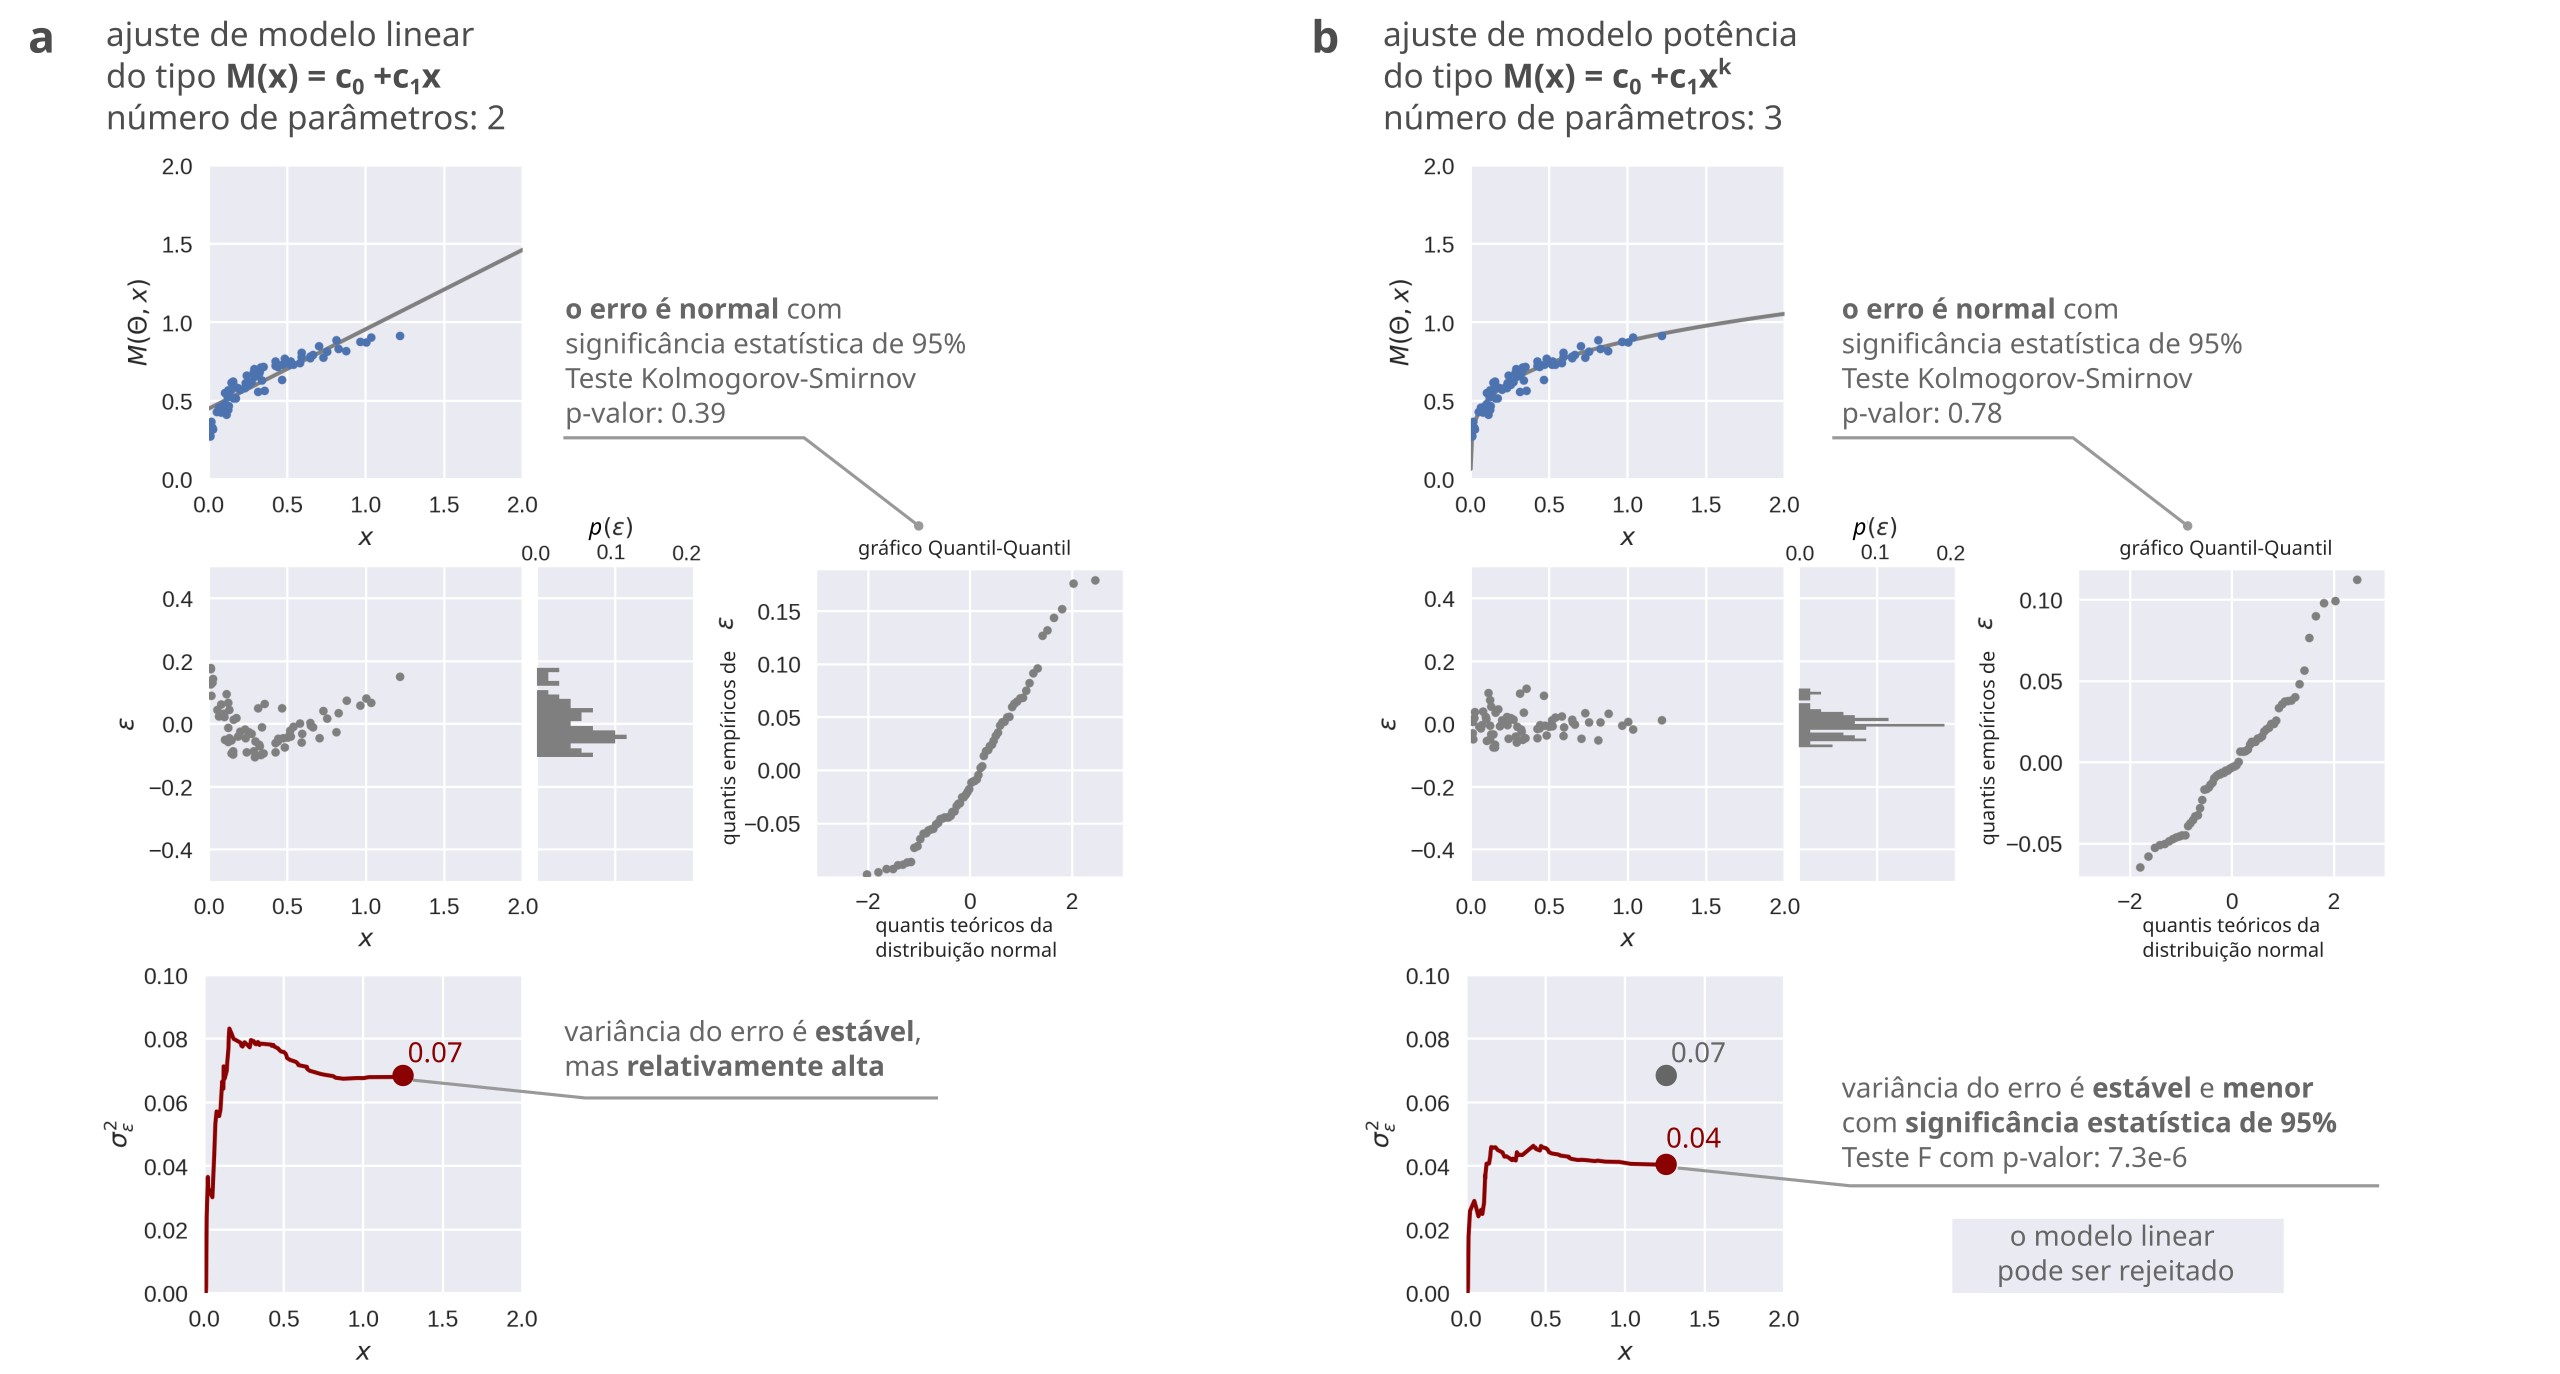
\includegraphics[width=0.95\linewidth]{fig_rejection.jpg}		
	\caption[Critérios de rejeição para seleção de modelos]
	{\textbf{---\;Critérios de rejeição para seleção de modelos.}
        \;\textbf{a}\;---\;Ajuste de um \gls{model} linear do tipo $M(x, \Theta) = c_{1}x + c_{0}$. \;\textbf{b}\;---\;Ajuste de um \gls{model} potência do tipo $M(x, \Theta) = c_{1}x^{k} + c_{0}$. Os dois modelos são ajustados para o mesmo conjunto de dados observados. Ambos os ajustes satisfazem as premissas de erro normal e variância estável (homoscedástica). Apenas pelo princípio da parcimônia (simplicidade), o \gls{model} linear deveria ser preferido pois apresenta menos \gls{parameters}. Mas o \gls{model} potência apresenta variância do erro menor com significância estatística de 95\%. Esse pode ser um critério de rejeição para o \gls{model} linear. 
	}
\label{fig:rejection}  % use qualitative label			
\end{figure}

\par O conceito de simplicidade de Popper faz sentido lógico, mas não responde exatamente como proceder diante de evidências observadas que apresentam ruído aleatório. Na prática, é impossível se obter dados perfeitamente aderentes a uma relação matemática fundamentada em algum princípio teórico, como uma função linear, quadrática, de potência, etc. Antes de prosseguir, aqui é importante diferenciar uma  \gls{teoria} de um \textbf{\gls{model-stats}}. As teorias estabelecem modelos matematicamente precisos sobre determinados fenômenos. Os modelos estatísticos, por outro lado, são um tipo de \gls{teoria} muito específica, que definem precisamente \textit{o padrão matemático de um conjunto de dados}, sem vínculos teóricos sobre os fenômenos subjacentes\footnote{Um exemplo intuitivo para essa diferença é considerar uma população, digamos, de mil triângulos com tamanhos aleatórios. Se olharmos os dados de perímetro e área, podemos facilmente criar um \gls{model-stats} entre essas duas variáveis: perímetros grandes em geral são acompanhados de áreas grandes. Mas isso não é uma lei teórica sobre os triângulos, pois alguns triângulos muito agudos apresentam grandes perímetros e área pequena. A \gls{teoria} matemática obviamente é que a área de um triângulo é a sua base vezes altura dividido por dois -- o perímetro está relacionado parcial e indiretamente.}. No caso das teorias, a questão em aberto na abordagem racionalista de Popper é quando que as anomalias nos dados devem ser levadas a sério a ponto de se rejeitar uma \gls{teoria} simples para dar lugar a uma \gls{teoria} mais complexa. Ou seja, o quanto que os dados devem se desviar do \gls{model} proposto pela \gls{teoria} para que ela seja considerada falseada pelas evidências? Essa pergunta inevitavelmente introduz uma decisão, que é a definição prévia de um \textbf{critério de rejeição}. A decisão sobre o critério de rejeição precisa ser \textit{antes} da avaliação da \gls{teoria} (\textit{a priori}) porque se for \textit{depois} nada impede que a \gls{teoria} nunca seja rejeitada -- basta estabelecer um critério sabidamente brando. O próprio Popper critica as teorias que, diante de evidências claramente falseadoras, usam de subterfúgios e explicações auxiliares \textit{ad hoc} para tentar sobreviver. Esse dilema fica evidente no caso das premissas mencionadas na Seção \ref{sec:epis:bayes} sobre o \gls{model-stats} do ruído aleatório: média nula, variância constante, independência no tempo e distribuição normal. Por exemplo, pode-se avaliar a premissa de normalidade do erro $\varepsilon$ a partir do gráfico Quantil-Quantil ou com testes de \gls{hipotese}, como o teste de Kolmogorov–Smirnov. No caso do gráfico Quantil-Quantil, a interpretação é puramente visual. Se o gráfico se desviar muito de uma linha reta, a premissa deve ser rejeitada. Já no caso do teste de \gls{hipotese}, o nível de confiança para a \gls{hipotese} nula é definido \textit{a priori}. Se o nível de confiança desejado for definido em 95\%, um p-valor menor ou igual que 0.05 quer dizer que a probabilidade da normalidade diante dos dados considerados é menor que 5\%, e a premissa deve ser rejeitada. Existe justificativa lógica para o nível de 95\%? Não existe. Outro exemplo, ilustrado na Figura \ref{fig:rejection}, é quando todas as premissas sobre os resíduos são satisfeitas tanto por um \gls{model} simples quanto por um \gls{model} complexo, mas o \gls{model} complexo é mais \textit{acurado} que o \gls{model} simples, ou seja, a dispersão do erro é \textit{menor}. O quanto a dispersão deve ser menor para se rejeitar o \gls{model} mais simples? De novo, é possível aplicar um teste de \gls{hipotese} para variâncias iguais, o Teste-F, e se obter uma resposta para um nível de confiança definido previamente. Se as variâncias forem diferentes com significância estatística, deve-se rejeitar o \gls{model} mais simples. De uma forma ou de outra, existe subjetividade envolvida na rejeição, pois são necessários critérios ou limiares definidos \textit{a priori}.

\section{Paradigmas} \label{sec:epis:kuhn}

\par Na Filosofia da Ciência, existe uma diferença importante entre o \textbf{\gls{contexto-justificacao}} e o \textbf{\gls{contexto-descoberta}}. O primeiro contexto trata do problema epistemológico de como justificar a verdade de uma \gls{teoria}. O segundo contexto investiga o problema histórico e sociológico de como se dá o progresso na Ciência – se é que existe progresso. As diferentes correntes filosóficas citadas nas seções anteriores se enquadram no primeiro contexto, pois oferecem soluções para o problema epistemológico da justificação. De uma forma ou de outra, elas conferem um papel importante para as evidências empíricas. Para os empiristas bayesianos, as evidências seriam utilizadas indutivamente para confirmar o \gls{grau-convic} em uma \gls{teoria} a partir da matemática das probabilidades. Para os racionalistas críticos, as evidências seriam essenciais para falsear teorias a partir da lógica dedutiva, deixando as teorias em uma eterna condição provisória – elas seriam corroboradas mas nunca confirmadas. A \textit{confirmação} e a \textit{rejeição}, assim, formam uma dicotomia um tanto paradoxal, pois ambas fazem sentido na prática da Ciência, mas se contradizem. Esse paradoxo é eliminado pela perspectiva do \gls{contexto-descoberta}. Em sua obra \textit{A estrutura das revoluções científicas}, Thomas Kuhn (1922-1996) traz uma contribuição substancial nesse sentido. 

\par Como historiador, Kuhn adverte que a Ciência não existe pairando no nada: ao contrário, é constituída por uma \textit{comunidade} de seres humanos que interagem ao longo da História, por sucessivas gerações, dentro de uma sociedade maior. A existência da \textbf{\gls{comunidade-cientifica}} implica que deve-se levar em conta não apenas a História da Ciência mas também a Sociologia da Ciência para entender o \gls{contexto-descoberta}. Essa comunidade obviamente não é um bloco único, mas uma rede social de comunidades menores, de diferentes disciplinas e áreas do conhecimento. Nessa linha, Kuhn propõe que a dinâmica de uma dada \gls{comunidade-cientifica} produz um padrão histórico cíclico, estruturado por três fases encadeadas: o período da \textbf{\gls{ciencia-normal}}, o período de \textbf{crise} e o período \textbf{revolucionário}. A confirmação e falsificação de teorias, portanto, predominam em diferentes etapas desse padrão histórico, sendo a confirmação um processo dominante no período da \gls{ciencia-normal} e a rejeição uma característica essencial do período de crise. Mas o processo mais importante para mudança na Ciência, que ocorre durante o período revolucionário, é a \textbf{competição} entre teorias. Em suas palavras:

\begin{adjustwidth}{100pt}{0pt}
\medskip
\small (...) a competição entre segmentos da \gls{comunidade-cientifica} é o único processo histórico que realmente resulta na rejeição de uma \gls{teoria} anteriormente aceitável ou na adoção de outra. -- Thomas Kuhn \cite{kuhn2012structure}.
\medskip
\end{adjustwidth}

\noindent Esse processo é inevitavelmente intergeracional, pois novos membros da comunidade precisam ser reeducados a pensar sob uma nova visão de mundo. Para ilustrar esse ponto, Kuhn cita um trecho marcante da autobiografia do físico Max Planck (1858-1947):

\begin{adjustwidth}{100pt}{0pt}
\medskip
\small (...) uma nova verdade científica não triunfa por convencer seus oponentes e fazê-los ver a luz, mas sim porque seus oponentes acabam eventualmente morrendo e uma nova geração cresce familiarizada com ela. -- Max Planck \textit{apud} Thomas Kuhn \cite{kuhn2012structure}.
\medskip
\end{adjustwidth}

\par Uma ideia chave para Kuhn é a de que uma \gls{comunidade-cientifica} compartilha um mesmo \textbf{\gls{paradigma}}. Por \gls{paradigma}, ele se refere a um conjunto de soluções exemplares para problemas de pesquisa, ou seja, um \gls{system} de teorias, instrumentos e práticas auxiliares que resolvem muito bem certos problemas amplamente aceitos e são \textit{promissores} para resolver problemas misteriosos e controversos com grande apelo competitivo. Esse apelo competitivo é importantíssimo, pois a atração de segmentos da comunidade em torno de um \gls{paradigma} apresenta uma \gls{feedback} positiva: quanto mais segmentos adotam o \gls{paradigma}, mais novos segmentos se convencem de que precisam adotá-lo também, sob a penalidade de ficar para trás. A \gls{comunidade-cientifica} no período normal, assim, opera tanto nas frentes teóricas quanto nas frentes aplicadas no sentido de reafirmar e articular o \gls{paradigma} hegemônico. Não se faz pesquisa científica nesse período com o objetivo explícito de encontrar novidades inesperadas, e o sucesso de uma pesquisa normal \textit{define-se justamente por não encontrar nenhuma surpresa}. Uma pesquisa bem sucedida geralmente confirma o que o \gls{paradigma} vigente já prometia ao trazer um detalhamento mais refinado ou ao expandir o campo de aplicações (por exemplo, pela invenção de novas tecnologias). Como em um jogo de quebra-cabeça, na \gls{ciencia-normal} se presume de antemão a imagem completa que as peças formam – o único desafio é fazer as peças se encaixarem. Aqui, surge a sensação de que a Ciência é um empreendimento \textit{cumulativo}: cada novo membro introduzido na \gls{comunidade-cientifica} teria a humilde missão de assentar mais um pequeno tijolo em um grande \say{edifício do conhecimento humano}. Na opinião de Kuhn, essa impressão de acumulação, além de equivocada no contexto maior, é reforçada pelo amplo uso de livros-texto na formação de novos pesquisadores. Esses livros didáticos funcionam como veículos da perpetuação do \gls{paradigma} hegemônico porque, quando não são simplesmente escritos de forma anti-histórica, eles distorcem a História para que ela pareça um processo linear e inevitável na direção das teorias vigentes.

\par Kuhn argumenta, com diversos exemplos na História da Ciência, que as peças do quebra-cabeça estudado pela \gls{ciencia-normal} eventualmente não se encaixam. Se por um lado o conhecimento se acumula durante o período normal, por outro também se acumulam \textbf{anomalias} empíricas e teóricas. Normalmente evitadas ou ignoradas, em dado momento essas anomalias passam a causar um mal-estar generalizado na \gls{comunidade-cientifica}, que entra então no período de crise. O exemplo de crise mais detalhado por Kuhn é a do geocentrismo, mas também ele oferece exemplos na química, na mecânica e no eletromagnetismo. Por esse ângulo, a História mostra que algumas crises se instalam lentamente, como na química, e que outras são súbitas, como a causada por Einstein na Física. Uma \gls{comunidade-cientifica} em crise apresenta diversos sintomas, tais como a discórdia, o descontentamento, debates filosóficos e, principalmente, a proliferação generalizada de teorias candidatas para explicar as anomalias.

\par A única saída para a crise é a revolução causada pela proposição de um \gls{paradigma} que seja irresistível para a \gls{comunidade-cientifica}. Como já assinalado, o novo \gls{paradigma} deve ser eficaz na solução de problemas já conhecidos e fazer promessas tentadoras para a solução dos problemas em aberto. As novas ideias devem, de alguma forma, oferecer uma \textbf{retrocompatibilidade} com as ideais antigas sem, contudo, serem contaminadas pelos problemas embutidos nos princípios fundamentais das ideias antigas. As revoluções científicas, assim, são episódios em que o suposto edifício do conhecimento é demolido para que uma nova edificação seja erigida sobre uma nova fundação, com uma nova planta. Nesse período revolucionário, que geralmente dura uma geração, a \gls{comunidade-cientifica} migra em massa para o novo \gls{paradigma}. Novos livros-texto são então escritos e se instala um novo ciclo histórico de \gls{ciencia-normal}. Um aspecto importante desse processo é que, para Kuhn, um \gls{paradigma} novo é tão diferente em termos de fundamentos do antigo que eles são \textit{incomensuráveis}: a comunicação intelectual entre eles é extremamente precária, pois representam diferentes visões de mundo. Exemplos típicos de \textbf{\gls{incomensu-theory}} ocorrem com o conceitos de massa, espaço e tempo na física de Newton e na física de Einstein. Apesar do mesmo nome e o mesmo símbolo, esses conceitos apresentam significados distintos sob os diferentes paradigmas, com implicações teóricas distintas\footnote{No \gls{paradigma} newtoniano a gravidade é uma força de atração relacionada à massa que atua de forma instantânea e à distância. Já no \gls{paradigma} einsteniano a gravidade não é uma força, mas uma \textit{consequência} da distorção do próprio espaço, implicando na existência de ondas gravitacionais. Para Kuhn, Einstein não simplesmente extrapola os limites de Newton: ele produz uma nova visão de mundo que é inconciliável com a anterior.}. Com isso, Kuhn traz uma conclusão inquietante: a de que \textit{não há progresso absoluto} na Ciência na direção da verdade sobre a realidade, apenas \textit{relativo} ao que estamos preocupados em explicar. Mais do que isso, com a sua tese, Kuhn aponta a profundidade da dinâmica social sobre a Ciência, que frequentemente é retratada como o mais racional dos empreendimentos humanos\footnote{A ênfase de Kuhn na relatividade do conhecimento, na contingência histórica e na presença de paradigmas deu fôlego para o surgimento da corrente filosófica do \textbf{pós-modernismo}, trazendo consigo a noção de que o conhecimento humano é um \textbf{discurso}. Assim, os pós-modernistas rejeitam grandes narrativas absolutistas e ressaltam a influência linguística, cultural e sobretudo política que permeia a produção de conhecimento.}.

\par Como foi exposto, a tese de Thomas Kuhn sobre o \gls{contexto-descoberta} elimina o paradoxo entre confirmação e rejeição, que são soluções contraditórias no \gls{contexto-justificacao}. Mas um olhar cauteloso capta que a abordagem de Kuhn é essencialmente empirista: ele busca \textit{confirmar} as ideias de paradigmas e de revoluções científicas a partir de exemplos da História da Ciência, ou seja, a partir de \textit{evidências empíricas}. Kuhn utiliza a \gls{infer-indu} para justificar uma \gls{teoria} sobre o \gls{contexto-descoberta}. Pela perspectiva racionalista crítica, por mais bem corroborada que seja, um único contra-exemplo seria suficiente para falsear a \gls{teoria} de Kuhn. O problema é que esse fato, paradoxalmente, \textit{ressuscita a dicotomia entre confirmação e falsificação}. Para piorar, se a \gls{teoria} de Kuhn é científica (ou seja, falseável), não seria ela \textit{em si} um \gls{paradigma} de como explicar o \gls{contexto-descoberta}? Surge aqui um laço recursivo de auto-referência. A recursão em um argumento geralmente é indicador do \gls{problem-regress}, mencionado anteriormente. Essa é uma típica situação aterrorizante de se estar andando eternamente em círculos que a Filosofia proporciona. Karl Popper, talvez por ser um filósofo e não um historiador, parece ter antevisto esses problemas e pré-estabeleceu que a \gls{teoria} sobre método científico não pode ser ela mesma científica -- falseável por evidências -- mas apenas uma \gls{teoria} baseada na Lógica.

\section{Subdeterminação} \label{sec:epis:under}

% introduzir o conceito de \gls{realism} científico
\par O que vimos até o momento insere-se na corrente filosófica mais ampla chamada de \textbf{\gls{realism-sci}}. Essa corrente essencialmente defende a tese de que o propósito da Ciência é providenciar teorias que são descrições verdadeiras da realidade \cite{bas1980}. Por exemplo, iniciamos este capítulo mencionando que Keith Beven classifica de \textit{\gls{realism} pragmático} a filosofia da maioria dos usuários de modelos hidrológicos, que é o entendimento tácito de que os modelos asseguram uma descrição aproximada da realidade que pode ser melhorada com novas tecnologias. O \gls{prag-realism}, para Beven, seria uma vertente do \gls{realism-sci}. As origens do \gls{realism-sci} podem ser identificadas nas ideias de René Descartes \cite{Agazzi2017}. Aqui, é preciso estabelecer que o \textbf{\gls{realism}} em si consiste na concepção da Metafísica que admite a existência da realidade \textit{objetiva}, ou seja, que o mundo não depende de ninguém para observá-lo. Nesse sentido, quando uma pessoa entra em uma sala e observa uma mesa, se admite que a mesa estava ali antes dela entrar. A mesa não se realizou instantaneamente no ato de observar. Objetos, como mesas, existem de forma independente dos sujeitos. Essa concepção se opõe ao \textbf{\gls{idealism}}, corrente que considera a realidade estritamente como um produto dos sujeitos, ou seja, \textit{subjetivo}. Se concordamos com a existência de um suposto objeto, como uma mesa, é por que ela se realiza de forma similar em nossas mentes, ou seja, \textit{intersubjetivamente}. Descartes flerta com o \gls{idealism} quando ele questiona a sua própria existência no \textit{Discurso do método}, em especial com a vertente do solipsismo -- a ideia de que a mente de quem está lendo este texto é a única coisa que de fato existe. Descartes basicamente aponta que, apesar de termos certeza absoluta sobre as ideias em nossa mente, é difícil garantir que elas correspondam à realidade externa. Nos termos dele, \textit{\gls{likelihood} não implica verdade}. Para tentar resolver esse problema, Descartes descreve o método da dúvida, que serviu de inspiração para a formação do método científico moderno, contribuindo para o debate em torno do \gls{problem-just} que abordamos até agora. No final das contas, o \gls{problem-just} está inerentemente contaminado pelo \textit{pressuposto de que a realidade objetiva existe}, sendo o conceito de \textbf{verdade} precisamente a \textit{correspondência} entre as teorias e a realidade.

\par A tese do \gls{realism-sci} parece óbvia, mas não é tão simples assim de defendê-la. De fato, Bas van Fraassen \cite{bas1980} e Nancy Cartwright \cite{nancy1983} fazem uma crítica profunda, propondo um ponto de vista radicalmente empirista denominado \textbf{\gls{instrument}}\footnote{Instrumentalismo é uma denominação  abrangente e neutra. Por exemplo, van Fraassen auto-denomina sua tese de \textit{\gls{empiricism} construtivista}. Os realistas, por sua vez, classificam o \gls{instrument} de \textit{anti-realismo}.} \cite{sep-constructive-empiricism}. Ambos sustentam a tese de que o objetivo da Ciência é produzir teorias que apresentem \textit{adequação empírica} -- e nada além disso. Como adequação empírica não implica logicamente uma descrição verdadeira da realidade, a reivindicação do \gls{realism-sci} é ambiciosa demais em termos epistemológicos. Esse ponto de vista não nega a existência da realidade (não é uma corrente idealista): o que se nega é a ambição de se obter uma descrição verdadeira sobre a realidade. As teorias e seus modelos seriam somente \textit{instrumentos} úteis construídos por cientistas para explicar evidências empíricas. Um dos principais motivos para essa alegação é o \textbf{\gls{problem-subdet}}\footnote{Tradução livre do termo em inglês \textit{underdetermination}.}, que é a dificuldade de garantir que as evidências observadas determinem a verdade de uma \gls{teoria} sem que existam teorias empiricamente equivalentes \cite{sep-scientific-underdet}, \cite{Tulodziecki2017}. A orientação de Popper, de se preferir sempre a \gls{teoria} mais simples, só funciona bem para teorias completamente falseáveis pelas evidências empíricas. Isso não é o caso para a maior parte das teorias, que quase sempre postulam a existência \textit{entidades inobserváveis} para explicar fenômenos que são diretamente observáveis. Por exemplo, na Física se evoca a existência de elétrons e campos eletromagnéticos (inobserváveis) para explicar os raios e relâmpagos de uma tempestade (observáveis). Isso complica tudo, pois não importa qual for a maneira de detectar as entidades inobserváveis, como os campos eletromagnéticos, as evidências indiretas sempre estarão contaminadas com uma \textit{carga teórica embutida}\footnote{Tradução livre do conceito de \textit{theory-ladenness} em inglês.} que estabelece a existências dessas entidades em primeiro lugar. Esse tipo de abordagem teórica envolve um tipo de raciocínio não-dedutivo, chamado de \textbf{\gls{ibe}}\footnote{Tradução livre do termo em inglês \textit{inference to the best explanation}.}, ou abdução. Por não ser dedutivo, esse raciocínio não garante a verdade da sentença consequente e também está sujeito ao \gls{problem-indu} postulado por Hume. Assim, uma \gls{teoria} que instancia entidades inobserváveis paga o preço de ser subdeterminada pelas evidências empíricas observáveis.

\par Uma das principais defesas do \gls{realism-sci} consiste em evocar o sucesso da Ciência como evidência de que as teorias científicas, mesmo instanciando entidades inobserváveis, progridem para descrever a realidade de forma cada vez mais verdadeira \cite{saatsi2017}. Pela perspectiva racionalista crítica, ainda que a verdade última sobre a realidade esteja permanentemente protegida, a rejeição de teorias oportuniza o isolamento incremental do conjunto de ideias potencialmente verdadeiras. De fato, é inegável que as predições teóricas e as aplicações tecnológicas que a Ciência produziu nos últimos séculos são impressionantes e não têm precedentes históricos. Diante de todo esse sucesso, até soa um tanto absurdo considerar que a Ciência moderna não descreve a realidade. Apesar da \gls{ibe} não garantir uma implicação lógica, como corretamente assinalam os instrumentalistas, os defensores do \gls{realism-sci} argumentam que seria \textit{um milagre} extremamente improvável as teorias atuais estarem obtendo bons resultados por motivos errados. Entretanto, Donald Hoffman traz a possibilidade de que as teorias científicas descrevam com notável adequação empírica o comportamento de uma \textit{interface cognitiva} \cite{Hoffman2015}. Ele sustenta que sistemas cognitivos, quando submetidos à seleção natural, são pressionados a operar através da \textbf{\gls{heuristic}}. Ou seja, aqueles sistemas que compactam as informações necessárias para tomar decisões úteis ganham vantagem competitiva. A evolução desses sistemas resulta em uma interface perceptual otimizada para a sobrevivência e reprodução, mas cuja probabilidade de ser equivalente à realidade é \textit{precisamente zero}. Como \gls{analogy}, considere a interface gráfica de um computador. Nesse caso, podemos facilmente observar o comportamento de botões e ícones para identificar padrões sem saber nada sobre os mecanismos eletrônicos subjacentes. As informações da interface gráfica não dizem absolutamente nada sobre o \textit{hardware}.  Para Hoffman, a verdade sobre realidade pode simplesmente não ter nada a ver com espaço, tempo, energia, matéria, etc -- nos termos de Kant, essas seriam as categorias transcendentais que usamos para compactar e integrar informações perceptuais \footnote{Donald Hoffman subverte o \gls{paradigma} do fisicalismo material ao propor que a realidade não é constituída fundamentalmente de partículas subatômicas, mas sim de uma rede infinita de interações entre agentes conscientes \cite{Hoffman2023}. As interações desses agentes produzem interfaces cognitivas que eventualmente instanciam laços de auto-referência, ou seja, realizam um \textit{Self}, um \say{Eu}. Essa \gls{hipotese} explica ao mesmo tempo tanto por que experiências subjetivas existem (note que elas não são previstas dentro do fisicalismo material) quanto por que o \gls{realism} definitivamente não se sustenta na escala quânticas (as propriedades supostamente físicas são realizadas instantaneamente no ato de observar). Apesar rejeitar o fisicalismo, a \gls{hipotese} de Hoffman é científica, pois é falseável no sentido de que seu desenvolvimento matemático deve, obrigatoriamente, reprojetar as leis da Física como as conhecemos através da interface.}.  

\par O \gls{problem-subdet} tem implicações diretas e relevantes para usuários de modelos ambientais, incluindo modelos hidrológicos. Nesse contexto, Naomi Oreskes e colegas apontam que a subdeterminação ocorre porque diversos processos representados pelos modelos não são observáveis \textit{na prática}, ou seja, as informações sobre o \gls{system} modelado são \textit{incompletas} tanto no tempo quanto no espaço \cite{Oreskes1994}. Essa versão mais branda da subdeterminação também é denominada de \textbf{\gls{problem-equifinal}} \cite{Beven2006}. Por exemplo, considere o escoamento subterrâneo que ocorre em bacias hidrográficas. É evidente que esse processo existe: uma expedição de campo torna isso claro ao se observar diretamente as nascentes dos riachos, os locais onde a água subterrânea aflora para a superfície. Inclusive, piezômetros podem ser instalados para se monitorar o nível do lençol freático, o que traz mais evidências diretas sobre esse processo. Porém, a extensão e a dinâmica completa desses fluxos subterrâneos é impossível de se monitorar na prática, sendo observável apenas pontualmente. Oreskes \textit{et al.} argumentam que a parcialidade das informações torna os sistemas naturais modelados \textit{logicamente abertos}. Ao contrário de sistemas logicamente fechados, como algoritmos e equações matemáticas, eles apontam que é impossível verificar ou validar um \gls{system} logicamente aberto diante de \textit{circunstâncias extenuantes} que frequentemente garantem explicações empiricamente equivalentes, ou \textit{equifinais}. Isso é intuitivo: quando não temos informações completas sobre algum evento que observamos, é natural o surgimento de explicações rivais e igualmente válidas. Aliás, é justamente por esse motivo que experimentos científicos são projetados de forma a se reduzir a abertura lógica do \gls{system} avaliado, ou seja, reduzir a influência das circunstâncias extenuantes. Assim, os modelos de sistemas naturais se apresentam como uma \textbf{\gls{hipotese} principal} que precisa da ajuda de \textbf{\gls{aux-hyp}}, tais como \gls{parameters}, os \gls{input-data}, as escalas adotadas e, principalmente, as premissas teóricas subjacentes. Assim, surge um paradoxo: é justamente em razão da ausência de informações que se busca a aplicação de modelos em primeiro lugar. Se as informações já estivessem completamente disponíveis, dificilmente um \gls{model} seria relevante para a tomada de decisão. Mas sem as informações completas, um \gls{model} torna-se subdeterminado pelas evidências disponíveis -- o \gls{problem-subdet} na aplicação de modelos é inexorável.

\par Para Keith Beven, o reconhecimento do \gls{problem-subdet} na modelagem hidrológica traz consequências radicais para a confirmação de modelos diante das evidências observadas, que é a necessidade de se avaliar o \textbf{erro total} associado a um dado \gls{model} hidrológico \cite{Beven2005}. Por essa perspectiva, a Equação \eqref{eq:bayes-model} estaria incompleta, pois ali o erro $\varepsilon$ representa apenas o ruído aleatório relacionado às evidências observadas. É necessário incluir não somente a \textbf{\gls{uncert-stats}}, resultante exclusivamente do ruído amostral, mas também a \gls{uncert-episteme}, que decorre das \gls{aux-hyp} necessárias para endereçar o \gls{problem-subdet} \cite{Beven2016}. Sendo assim, a \textbf{\gls{eq-total-error}} para modelos hidrológicos apresenta a seguinte forma:
\begin{linenomath*}
\begin{equation}
\label{eq:total-error}
    O(x, t) + \varepsilon_{O}(x, t) + \varepsilon_{\Delta}(\Delta x,\Delta t, x, t) = M(\Theta, \Upsilon, \varepsilon_{\Upsilon}, x, t) + \varepsilon_{M}(\Theta, \Upsilon, \varepsilon_{\Upsilon}, x, t) + \varepsilon_r
\end{equation}
\end{linenomath*}
Em que $O(x, t)$ é a observação obtida na variável independente $x$\footnote{Em modelos hidrológicos a variável independente geralmente é o espaço bidimensional, ou seja, deve-se substituir $x$ por $x, y$.} e no tempo $t$; $\varepsilon_{O}(x, t)$ é o \textbf{\gls{error-measure}} da observação; $\varepsilon_{\Delta}(\Delta x,\Delta t, x, t)$ é o\textbf{ \gls{error-commensu}} na escala de modelagem $\Delta x$ e $\Delta t$; $M(\Theta, \Upsilon, \varepsilon_{\Upsilon}, x, t)$ é a predição do \gls{model} em $x, t$ a partir do vetor de \gls{parameters} $\Theta$, do vetor de \gls{input-data} $\Upsilon$ e do \textbf{\gls{error-input}} $\varepsilon_{\Upsilon}$; $\varepsilon_{M}(\Theta, \Upsilon, \varepsilon_{\Upsilon}, x, t)$ é o \textbf{\gls{error-struct}}, e; $\varepsilon_r$ é o \textbf{erro aleatório} remanescente. O \gls{error-commensu} $\varepsilon_{\Delta}$ resulta da conversão entre escalas, representando a \gls{uncert-episteme} da diferença de significado entre uma observação obtida pontualmente em \textit{x, t} e a variável correspondente modelada em $\Delta x, \Delta t$. Por exemplo, enquanto a vazão observada de um rio é instantânea e referente a uma seção específica do canal, a vazão modelada integra algum passo de tempo e se refere a uma extensão espacial discreta. O \gls{error-measure} $\varepsilon_{O}$ e o \gls{error-commensu} $\varepsilon_{\Delta}$ são mantidos do lado esquerdo da Equação \eqref{eq:total-error} para denotar que juntos eles compõe o \textbf{\gls{error-obs}}. Já o \gls{error-input} $\varepsilon_\Upsilon$ origina-se do agrupamento das incertezas tanto das condições de contorno (como os mapas da topografia, solos, vegetação, etc), quanto das variáveis forçantes do \gls{model} (como chuva, temperatura, velocidade do vento, etc). Nesse caso, a incerteza geralmente é estatística, de maneira que amostras representativas tendem a reduzir seu impacto. Ela pode, contudo, também assumir uma natureza epistêmica quando os dados de entradas correspondem a \textbf{cenários}, fato que agrega uma carga conceitual. Por fim, o \gls{error-struct} $\varepsilon_M$ resulta da \gls{uncert-episteme} da configuração teórica e numérica do \gls{model} hidrológico. Essa componente é fortemente influenciada pelas premissas teóricas previamente definidas sobre o \gls{system} e seus processos hidrológicos.
% figure
\begin{figure}[t!] % place figure in the page
	\centering				
	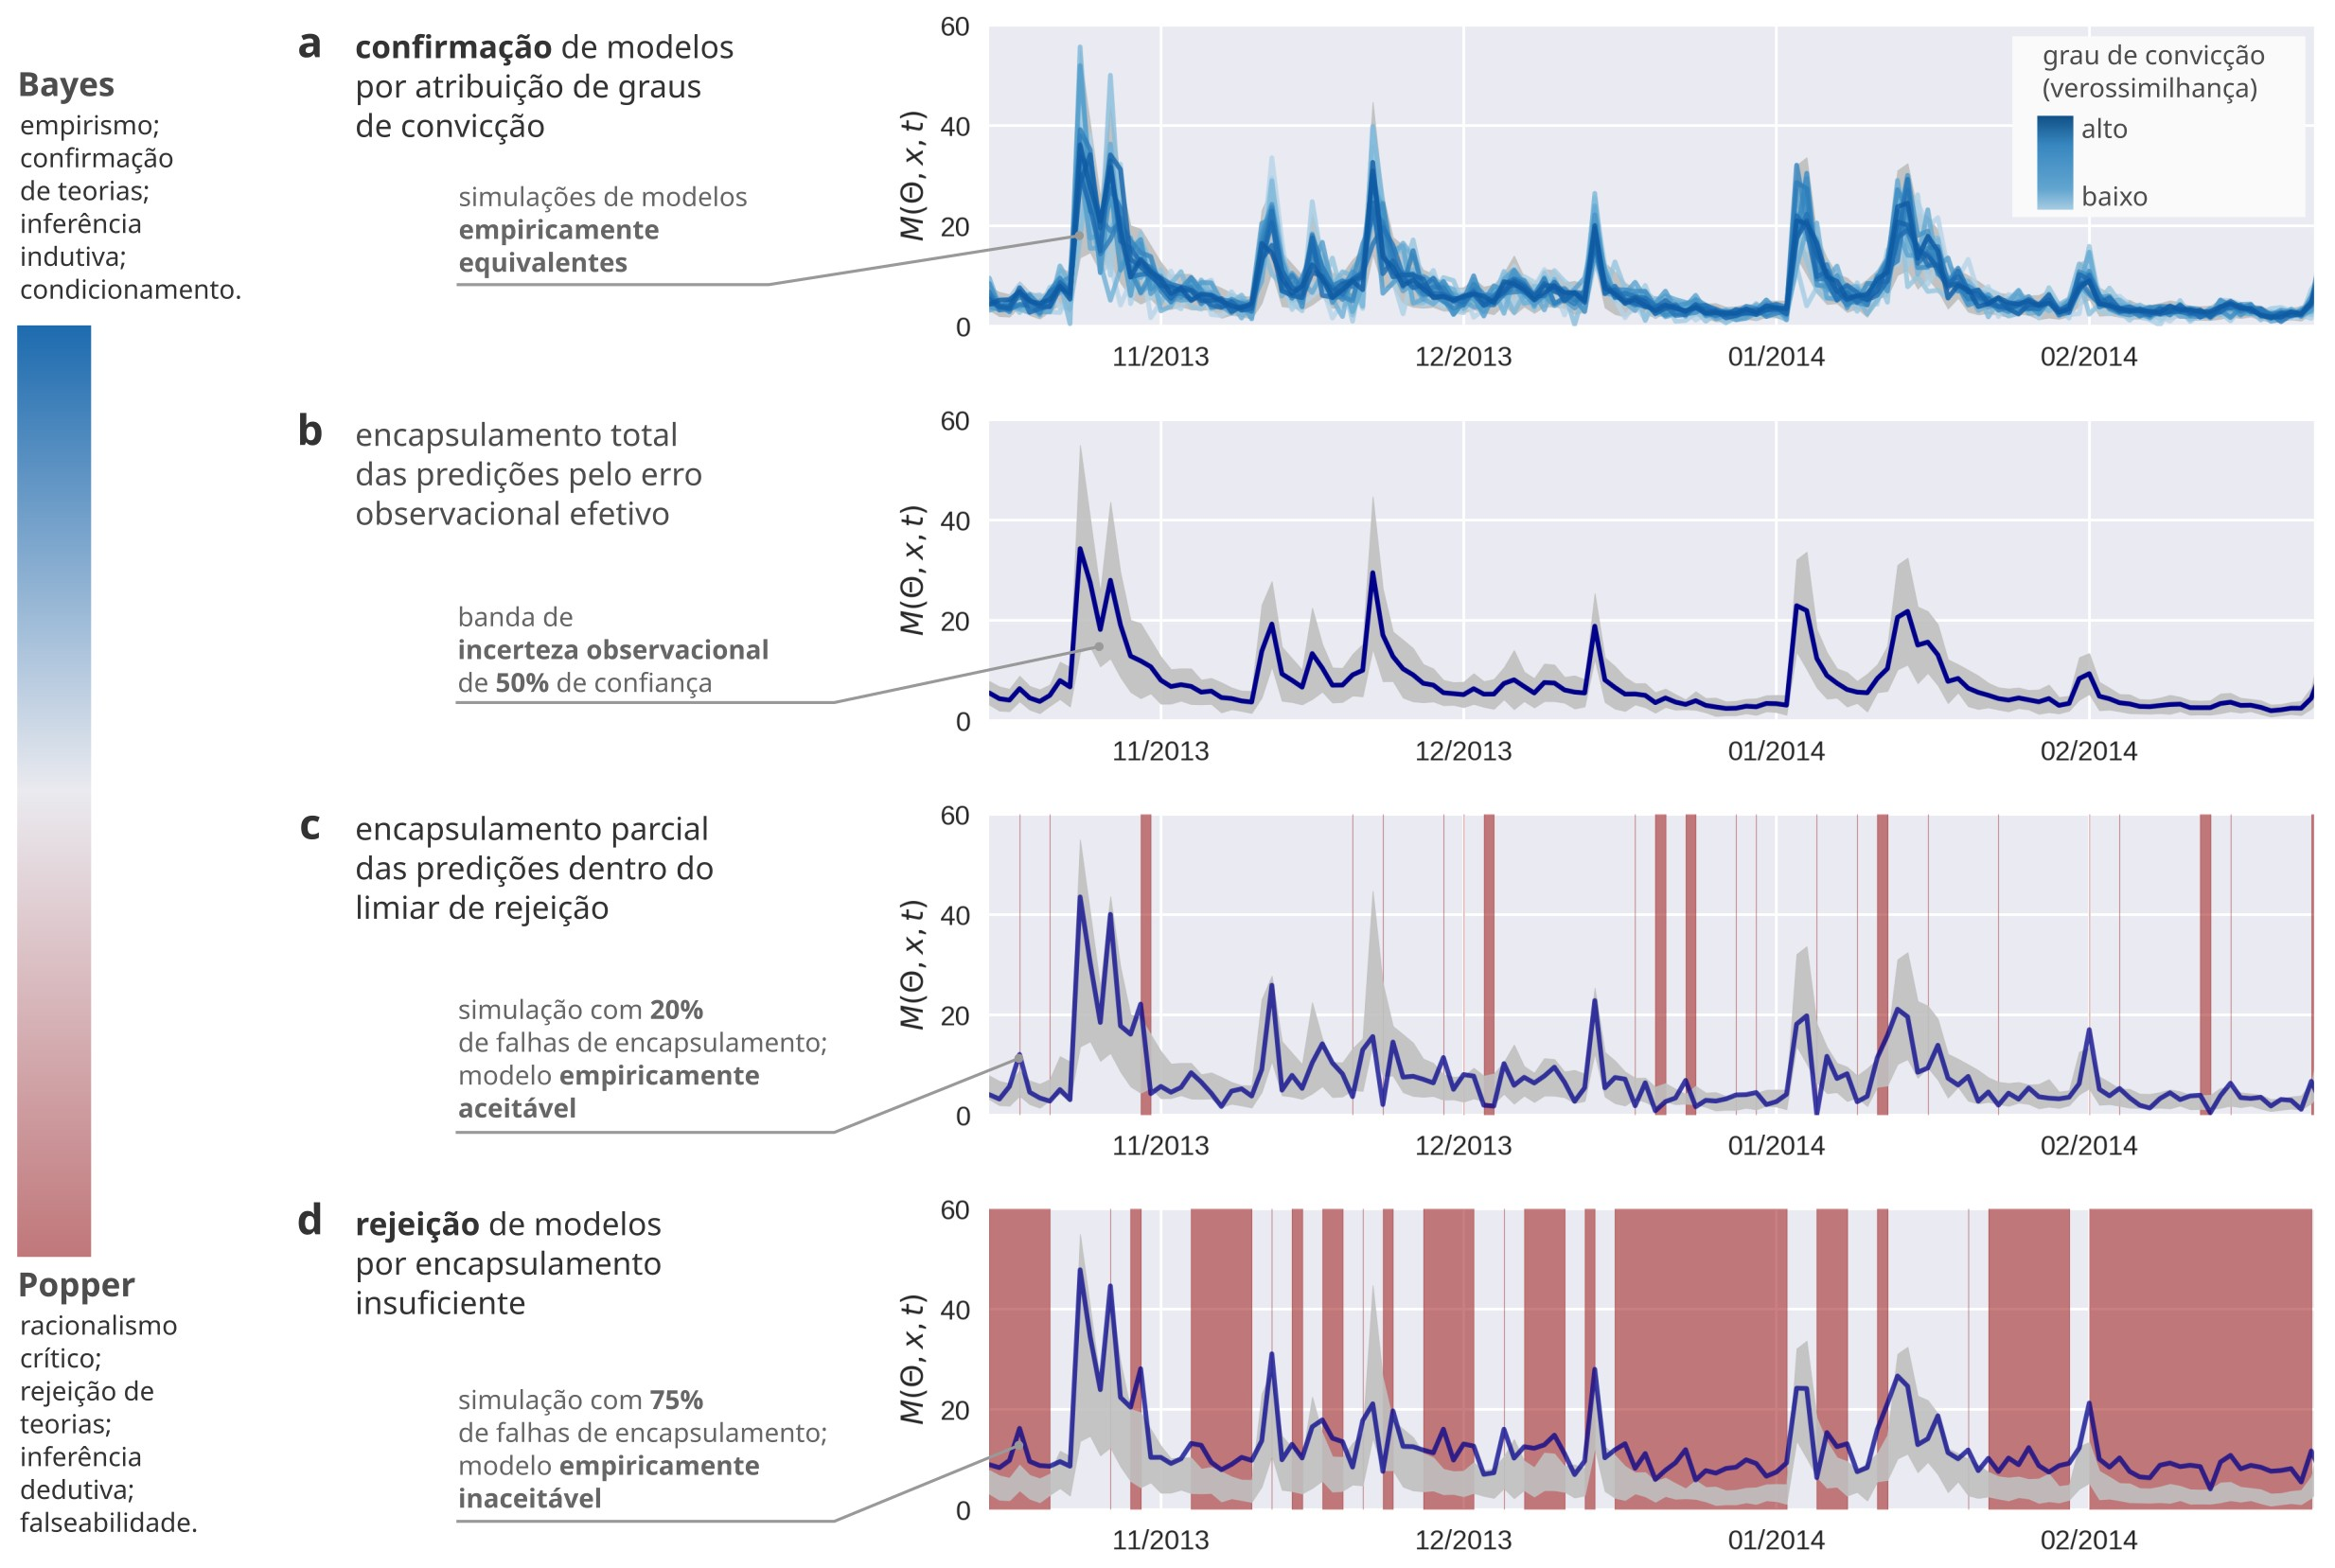
\includegraphics[width=0.95\linewidth]{fig_approach.jpg}		
	\caption[Abordagem instrumentalista para a modelagem hidrológica]
	{\textbf{---\;Abordagem instrumentalista para a modelagem hidrológica.}
        Nessa abordagem tanto a confirmação de Bayes quanto a rejeição de Popper são empregadas sob o reconhecimento do \gls{problem-subdet} (equifinalidade). \;\textbf{a}\;---\;Confirmação de modelos pelo \gls{conditioning} bayesiano, em que graus de confirmação (medidas de \gls{likelihood} informais) são atribuídos para \gls{emp-eq-model}. No caso, todos os modelos foram encapsulados pela banda de incerteza observacional dentro do limiar de rejeição pré-estabelecido.\;\textbf{b}\;---\;Encapsulamento total (sem falhas) de uma simulação (série temporal) pelo \gls{error-obs} das evidências empíricas. No caso ilustrado a banda de incerteza apresenta nível de confiança de 50\%. Uma banda mais ou menos abrangente deve ser definida \textit{a priori}.\;\textbf{c}\;---\;Encapsulamento parcial (com 20\% de falhas) de uma simulação pelo \gls{error-obs}. Como a banda é de 50\% de confiança, as falhas estão dentro do limiar de rejeição e o \gls{model} pode ser considerado empiricamente aceitável.\;\textbf{d}\;---\;Rejeição de modelos por encapsulamento insuficiente (75\% de falhas). Nesse caso as falhas superam o nível de 50\% de confiança e o \gls{model} deve considerado empiricamente inaceitável.\;
	}
\label{fig:approach}  % use qualitative label			
\end{figure}

% equação do encapsulamento
\par Com a Equação \eqref{eq:total-error}, Keith Beven operacionaliza um \gls{paradigma} instrumentalista para a modelagem hidrológica que, para além da confirmação, \textit{admite a rejeição de modelos}. Essa abordagem segue as recomendações discutidas por Albert Tarantola, de considerar tanto a confirmação empirista de Bayes quanto a rejeição racionalista de Popper para uma abordagem filosoficamente explícita de modelagem ambiental \cite{Tarantola2006}. Nessa linha, a crítica sobre o \gls{paradigma} hegemônico de modelagem, dominado pelo \gls{prag-realism}, é que a confirmação de modelos ocorre sob o preço de se subestimar as incertezas epistêmicas, mascarando elas em um erro aleatório que é minimizado pelo ajuste de técnicas de otimização, como na Equação \eqref{eq:bayes-model}. Isso conduz ao \textbf{\gls{problem-overfitting}} do modelos aos dados disponíveis que foram utilizados. Através do \textbf{\gls{proc-calib}} convencional\footnote{Também denominado de \textit{problema invertido}}, chega-se na conclusão (equivocada) de que o \gls{model} ajustado que foi identificado consiste na única representação empiricamente adequada. Por outro lado, a nova abordagem instrumentalista, nas palavras de Beven:

\begin{adjustwidth}{100pt}{0pt}
\medskip
\small (...) consiste em aceitar que é muito implausível que as estruturas de nossos modelos atuais sejam descrições realisticamente verdadeiras dos sistemas ambientais de interesse, de maneira que talvez existam muitos outras configurações que produzam predições aceitavelmente consistentes com quaisquer dados observados disponíveis. Isso consiste em tratar o problema da identificabilidade como um problema de equifinalidade de estruturas e \gls{parameters} de modelos em reproduzir o comportamento conhecido do \gls{system}.\footnote{Tradução livre de: \textit{There is, however, another approach. That is to accept that it is very unlikely that our current model structures are truly realistic descriptions of the enviromental systems of interest so that there may indeed be many different models that can be shown to provide predictions that are acceptably consistent with whatever observed data are available. That is to treat the problem of identifiability as one of equifinality of model structures and parameter sets in reproducing the known behaviour of the system}.} -- Keith Beven (2009. p. 15) \cite{Beven2009}.
\medskip
\end{adjustwidth}

\noindent É importante assinalar que essa nova abordagem não abandona o processo de confirmação pelo método de \gls{conditioning} bayesiano da distribuição posterior dos \gls{parameters} $\Theta$. Ainda que a \gls{eq-total-error} torne impossível um tratamento formal da \gls{likelihood} $P(O|M)$, permanece possível a atribuição de diferentes graus de convicção, ou pesos, para os \textbf{\gls{emp-eq-model}} por medidas de \gls{likelihood} informais $\mathcal{L}(O|M)$. A novidade da abordagem consiste em estabelecer que um \textbf{\gls{emp-acc-model}}\footnote{Keith Beven se refere a modelos empiricamente aceitáveis por \textit{behaviroural models}.} ocorre quando o seu erro estrutural $\varepsilon_M$ for menor que o seu \gls{error-obs} $\varepsilon_O + \varepsilon_{\Delta}$. Do contrário, o \gls{model} deve ser rejeitado. Isso implica que as predições de um \gls{model} qualquer devem ser \textit{encapsuladas}\footnote{Tradução livre do termo \textit{bracketing} em inglês.} por um intervalo de confiança definido \textit{a priori} como um critério de rejeição. Ou seja, para um nível de confiança de $\alpha$\%, a \textbf{\gls{eq-bracketing}}:
\begin{linenomath*}
\begin{equation}
\label{eq:bracketing}
    O_{100-\alpha\%}(x, t) < M(\Theta, \Upsilon, \varepsilon_{\Upsilon}, x, t) < O_{\alpha\%}(x, t) \quad \forall \quad x, t
\end{equation}
\end{linenomath*}
deve ser válida com uma frequência de pelo menos $\alpha\%$; em que $O_{100-\alpha\%}$ e  $O_{\alpha\%}$ são os limiares inferiores e superiores do intervalo de confiança do \gls{error-obs} em cada ponto amostral $x, t$. Essa abordagem tem exatamente a mesma estrutura dos testes de \gls{hipotese} estatísticos: 1) se define previamente um critério de rejeição por um nível de confiança $\alpha$\%; 2) se calcula uma estatística de teste, no caso a taxa de encapsulamento da simulação, e; 3) se avalia o p-valor do teste, que no caso é a taxa de falhas de encapsulamento. Se o p-valor for maior que o nível de confiança, deve-se rejeitar o \gls{model}. Por outro lado, todos os modelos que passarem pelo teste de encapsulamento mínimo são tidos como empiricamente equivalentes e podem ser confirmados com base em medidas de \gls{likelihood}. A Figura \ref{fig:approach} ilustra a abordagem para o encapsulamento de uma série temporal de uma variável hidrológica qualquer, mas que geralmente é a vazão em uma seção de rio. Nota-se que pré-definição do nível de confiança implica em bandas de incerteza observacional mais ou menos abrangentes. Esse fato introduz o seguinte dilema: quando se deseja muita certeza sobre as predições, a banda observacional pode ser muito larga, resultando em diversas simulações empiricamente aceitáveis e pouca precisão do erro estrutural. Isso cria a necessidade de se obter mais evidências, de forma que as observações em si apresentem bandas estreitas para níveis altos de confiança. Outro aspecto diferente do \gls{paradigma} hegemônico, que opera unicamente pela confirmação, nada impede a eventual \textit{rejeição de todos os modelos testados} pela \gls{eq-bracketing}. Se for o caso, Beven salienta, surge uma oportunidade valiosa para transformar a modelagem em um processo de aprendizado, que obriga os usuários a revisar detalhadamente tanto as \gls{aux-hyp} quanto a \gls{hipotese} principal, ou seja, as próprias premissas teóricas adotadas na concepção dos processos hidrológicos modelados. No limite, a rejeição total impõe a necessidade de novas teorias e explicações \cite{Beven2018}. Sem isso, a \gls{comunidade-cientifica} desse campo estará eternamente presa aos mesmos paradigmas. $\blacksquare$

\clearpage

\section{Resumo do capítulo} \label{sec:epis:summary}

\par Este capítulo buscou estabelecer os fundamentos de uma filosofia instrumentalista para a aplicação de modelos hidrológicos. Essa filosofia entende que a tomada de decisão baseada em evidências deve ser auxiliada por informações sobre a \gls{uncert-empirical} inerente ao uso de modelos. Nesse sentido, é preciso uma atitude crítica diante do que os modelos hidrológicos literalmente são (tensões em circuitos eletrônicos) e o que os usuários de modelos hidrológicos imaginam (processos hidrológicos em bacias hidrográficas). As principais conclusões são:

\begin{itemize}
    \item[$\blacksquare$] \textbf{O problema da justificação}. Existe uma dificuldade de se justificar a verdade de teorias, de se estabelecer explicações definitivas sobre os eventos e fenômenos. Por um lado, os racionalistas apelam para o uso de \gls{infer-dedu}, que garante a verdade de enunciados desde que suas premissas sejam verdadeiras. Por outro, os empiristas preferem usar a \gls{infer-indu}, que faz uso de evidências empíricas para generalizar padrões observados.
    \item  [$\blacksquare$] \textbf{Confirmação indutiva de hipóteses}. A epistemologia bayesiana descreve o processo de \gls{conditioning} empírico para confirmar hipóteses. Ao se reconhecer a existência de ruído aleatório nas observações empíricas, a verdade de uma \gls{hipotese} deve ser descrita como um \gls{grau-convic}, ou probabilidade. Nesse processo, a distribuição de probabilidade de hipóteses é incrementalmente ajustada a partir da aplicação do Teorema de Bayes. 
    \item[$\blacksquare$] \textbf{Rejeição dedutiva de teorias}. Karl Popper, ao analisar a Lógica da pesquisa científica, defende que a única forma segura de se adquirir conhecimento é pela refutação dedutiva. Nesse sentido, o papel das evidências empíricas consiste em testar uma \gls{hipotese} a partir de contra-exemplos que provam sua falsidade. Por esse motivo, Popper alega que as teorias científicas devem ser teorias falseáveis, que permitem sua própria rejeição.  
    \item     [$\blacksquare$] \textbf{Paradigmas e o contexto da descoberta}. Thomas Kuhn, ao explorar a História da Ciência, elimina a aparente contradição entre confirmação e rejeição de teorias. Ele sustenta que a dinâmica da \gls{comunidade-cientifica} desempenha um papel profundo na produção do conhecimento, especialmente no advento de paradigmas. Para ele, a confirmação ocorre em períodos de \gls{ciencia-normal}, enquanto que a rejeição predomina em períodos de crise. Os períodos de crise só acabam quando a competição de novas ideias dá lugar a um novo \gls{paradigma}.
    \item[$\blacksquare$] \textbf{O problema da subdeterminação}. O \gls{realism-sci} é profundamente questionado por Bas van Frassen e Nancy Cartwright. Eles estabelecem uma perspectiva instrumentalista, em que o objetivo da Ciência é unicamente produzir teorias empiricamente adequadas. Isso decorre principalmente da instância de entidades inobserváveis, fato que torna as teorias subdeterminadas pelas evidências. Uma versão disso ocorre na modelagem hidrológica pelo fato de muitos processos modelados não serem observáveis na prática -- o denominado \gls{problem-equifinal}. Nessa linha, Keith Beven propõe um \gls{paradigma} instrumentalista para a aplicação de modelos, que permite a rejeição de modelos a partir do teste de encapsulamento das predições pela incerteza observacional. Os modelos que passam no teste são tidos como empiricamente aceitáveis e equivalentes.  
\end{itemize}

\end{document}